%%%%%%%%%%%%%%%%%%%%%%%%%%%%%%%%%%%%%%%%%%%%%%%%%%%%%%%%%%%%%%%%%%%%%%%%%%%%%%%%
%									Chapter 3								   %
%%%%%%%%%%%%%%%%%%%%%%%%%%%%%%%%%%%%%%%%%%%%%%%%%%%%%%%%%%%%%%%%%%%%%%%%%%%%%%%%
\chapter{Side-Channel Attacks}
\label{chap:sca}
\citationChap{
	All models are wrong, but some models are useful.}{George Box}
\minitoc
\newpage
%%%%%%%%%%%%%%%%%%%%%%%%%%%%%%%%%%%%%%%%%%%%%%%%%%%%%%%%%%%%%%%%%%%%%%%%%%%%%%%%
\section{Definition of a Side-Channel Attack}
    \label{sec:attack_scenario}
    %%%%%%%%%%%%%%%%%%%%%%%%%%%%%%%%%%%%%%%%%%%%%%%%%%%%%%%%%%%%%%%%%%%%%%%%%%%%%%%%
%                           DEFINITION OF THE SCA ATTACK SCENARIO              %
%%%%%%%%%%%%%%%%%%%%%%%%%%%%%%%%%%%%%%%%%%%%%%%%%%%%%%%%%%%%%%%%%%%%%%%%%%%%%%%%
\subsection{The Attack Scenario}
\label{sec:problem_position}
Let \(\target\) be the instance of the \emph{target} device under an attack conducted by an adversary, \aka{} \emph{attacker}, denoted by \(\attacker\).
We assume that \(\target\) runs a cryptographic primitive \(\encrypt{}\) each time that a query, represented by a plaintext \(\ppp\), is sent by the attacker.
The primitive being set by a secret encryption key \(\kkkTest\), the target returns the ciphertext corresponding to the encryption of the sent plaintext, that is, \(\ccctx = \encrypt{\ppp, \kkkTest}\).
The goal of the attacker is then to guess the secret key, assumed to belong to a known key space \(\keySet\).

% Modelization
In this thesis, we modelize a \gls{sca} by the following scenario, that is illustrated in \autoref{fig:gray-box}.
\begin{figure}
    \centering
    \begin{tikzpicture}[>=stealth']
        % Locations
        \def\ClientToServer{++(6,0)}
        \def\ServerToClient{++(-6,0)}
        \def\Lifeline{++(0,-4.5)}
        % Lifelines
        \path (0,0)           node[draw] (Attacker) {\(\attacker\)}
              \ClientToServer node[draw] (Target) {\(\target\)};
        \draw (Attacker) -- \Lifeline (Target) -- \Lifeline;
        % Blocks
        \path (Target)
              ++(0,-1) node (BeginProcess) {}
              ++(0,-1) node (EndProcess)   {};
        % \filldraw[fill=blue!30] (BeginProcess.west) rectangle (EndProcess.east);
        % Calls 
        \draw[->] (BeginProcess)\ServerToClient -- node[above] {\(\ppp_1,\ldots,\ppp_{\numTracesAttack}\)} (BeginProcess);
        \draw[->] (EndProcess) -- node[above] {\(\ccctx_1, \ldots, \ccctx_{\numTracesAttack}, \textcolor{ceagray}{\xxx_1, \ldots, \xxx_{\numTracesAttack}}\)}\ServerToClient;
        \draw[->] (EndProcess) \ServerToClient ++(0,-1) -- node[above] {\(\disting{\attackSet}\)} \ClientToServer;
        % \draw[->] (EndProcess)\ServerToClient ++(0, -1) -- node[above] {\(\kkkHyp = \kkkTest\)?} \ClientToServer;
        \draw[->] (EndProcess) ++ (0, -2) -- node[above] {\(\guessVec{\disting{\attackSet}}[\keyTest]\)} \ServerToClient;
        \end{tikzpicture}
    \caption{Black: scenario of the black-box model.
    Grey: additional information added in the gray-box scenario.}
    \label{fig:gray-box}
\end{figure}
First, the target randomly draws a secret key \(\kkkTest\) that is used for the encryption.
Then, \(\attacker\) sends a given number \(\numTracesAttack\) of queries to the target \(\target\).
Those queries are materialized by the input plaintexts \(\ppp_1, \ldots, \ppp_{\numTracesAttack}\).
For each plaintext \(\ppp_i \in \plaintextSet\), the target \(\target\) returns the corresponding ciphertext \(\ccctx_i\) but also a measurement \(\xxx_i \in \leakSpace\), \aka{} \gls{sca} \emph{trace}, corresponding to the physical leakage occuring during the computation \(\ccctx_i = \encrypt{\ppp_i, \kkkTest}\).
In the remaining of this thesis, we denote by \(\attackSet \eqdef \-\{(\xxx_1, \ppp_1), \ldots, (\xxx_{\numTracesAttack}, \ppp_{\numTracesAttack})\}\) the \emph{attack set} acquired by the attacker \(\attacker\) during the \gls{sca}.
% Comment gray/black-box
This attack scenario is often called a \emph{gray-box} attack, in opposition to a black-box scenario corresponding to classical cryptanalysis, where the attacker does not have access to the \gls{sca} traces in the attack set, but rather the ciphertexts instead.

% Introducing probas
From a probabilistic point of view, \(\ppp, \kkkTest, \xxx\) can be respectively seen as the realizations of the corresponding random variables \(\PPP, \KKK, \XXX\), according to the probabilistic graph presented in \autoref{fig:proba_graph}.
\begin{figure}
    \centering
    \begin{tikzpicture}[rounded corners, >=stealth']
        \node[fill=cealightgray] (Plaintext) {\(\ppp_i \gets \PPP\)}; 
        \node[below = of Plaintext] (Ghost){};
        \node[fill=cealightgray, below = of Ghost] (Key) {\(\kkkTest \gets \KKK\)};
        \node[fill=cealightgray, right = of Ghost] (Sensitive) {\(\zzz_i = \miniEncrypt{\ppp_i, \kkkTest}\)};
        \node[fill=cealightgray, right = of Sensitive] (Leakage) {\(\xxx_i \gets \XXX \given \ZZZ = \zzz_i\)};
        % Dessin des liens
        \draw[->] (Plaintext) -- (Sensitive);
        \draw[->] (Key) -- (Sensitive);
        \draw[->] (Sensitive) -- (Leakage);
    \end{tikzpicture}
    \caption{Probabilistic graph denoting the links between the data.}
    \label{fig:proba_graph}
\end{figure}
More precisely, we make the assumption that \(\XXX\) only depends on a random variable \(\ZZZ\) resulting in an intermediate computation denoted by \(\miniEncrypt{}\) involving chunks of \(\PPP\) and \(\KKK\),%
\footnote{
    \autoref{sec:reducing_chunk} will discuss how to reduce the problem to chunks of plaintexts and keys.
}
\eg{}, \(\miniEncrypt{\PPP, \KKK} = \PPP \plusgf \KKK\).
This random variable is called \emph{sensitive} since it depends on the secret key, and \emph{intermediate} since it corresponds to an intermediate state between the plaintext and the final ciphertext.
In other words, some knowledge about the values \(\zzz_i = \miniEncrypt{\ppp_i, \kkkTest}, i \in \llbracket 1, \numTracesAttack \rrbracket\) of the sensitive intermediate variable, induces some knowledge about the underlying secret key \(\kkkTest\) used for the encryption.

Moreover, we assume that the couple \((\PPP, \XXX)\) is not independent from the secret key \(\KKK\).
Otherwise, considering the gray-box scenario has no further interest compared to the black-box one.
% Discussion continuous/discrete for the traces
Finally, the random variable \(\XXX\) is usually assumed to be drawn from a continuous \gls{pdf}, since it measures a physical phenomenon.
However in practice, the observations of this random variable are discretized during the acquisition phase by the oscilloscope.
That is why the leakage space is often of the type \(\leakSpace = \llbracket 0, 2^\omega-1 \rrbracket^\traceLength\), where \(\traceLength\) is the dimensionality of the observations, and where \(\omega\) denotes the resolution of the oscilloscope -- typically \(\omega=8\).

% Exploiting the information by the attacker
In the pursuit of his ultimate goal, the attacker can process the attack set in order to extract \emph{information} on (a chunk of) the secret key.
Depending on how the attacker wants to exploit this information, the latter one can take different forms.
\begin{itemize}
    \item Either the attacker aims at directly recovering the secret key from \(\attackSet\), without additional investigation.
    Then, he returns a value \(\kkkHyp\) that he believes to correspond to the right key \(\kkkTest\), according to the extracted information from \(\attackSet\).
    \item Or the attacker \(\attacker\) may want to combine a \gls{sca} with other attack techniques such as:
    \begin{itemize}
        \item \emph{Algebraic} attacks, \eg{}, by using a \gls{sat} solver to find the right key among a restricted list of \(\succOrder\) key candidates \(\kkkHyp_1, \ldots, \kkkHyp_\succOrder\) returned after the \gls{sca} -- where \(\succOrder \ll \card{\keySet}\).
        Such techniques have been initially introduced by Renauld \etal{}~\cite{renauld_algebraic_2009,renauld_aes_2009}.%
        \footnote{
            This approach has been rewarded at the \textsc{Ches} 2018 \gls{ctf}~\cite{gohr_ches_2019,hu_machine_2019,gohr_efficient_2020}.
        }
        \item \emph{Brute-force} attacks, \eg{}, by using a key enumeration algorithm~\cite{veyrat-charvillon_optimal_2012,martin_counting_2015,bogdanov_fast_2015,poussier_key_2018} fed with the set of key hypotheses \(\keySet\) sorted in a decreasing order of preference, returned by the \gls{sca} until it reaches the right key \(\kkkTest\).
    \end{itemize}
\end{itemize}

More generally, those different approaches may be encompassed by the following one: the \gls{sca} attacker \(\attacker\) returns a vector assigning a score to each hypothetical value of the key.
This vector is computed thanks to a so-called \emph{distinguisher} that we define hereafter.
\begin{definition}[Distinguisher]
    \label{def:distinguisher}
    Let \(\attackSet\) be an attack set.
    A \emph{distinguisher} is a mapping from \(\attackSet\) to a \emph{score vector} in \(\realSet^{\card{\keySet}}\):
    \begin{equation}
        \disting{}: \attackSet \mapsto 
        \left(
        \begin{matrix}
			\vdots \\
			\disting{\attackSet}[\kkk] \\
			\vdots
        \end{matrix}
        \right).
    \end{equation}
\end{definition}
\begin{remark}
    The definition of the distinguisher may be refined by constraining the scores to belong to the interval \([0,1]\), \(0\) denoting the least confidence in the corresponding key hypothesis while \(1\) denoting the greatest confidence.
    This constraint can still be obtained by applying a normalization of the scores.
\end{remark}
% Interpretation of the distinguisher on the other scenarios
This definition encompasses the different forms of information exploitation from the \gls{sca} presented so far.
For the first way, the attacker \(\attacker\) takes \(\kkkHyp = \argmax_{\kkk \in \keySet} \disting{\attackSet}[\kkk]\).
The attack is then said \emph{successful} \gls{iff} \(\kkkHyp = \kkkTest\).
For the second way, \ie{} the algebraic attack, the attacker \(\attacker\) returns a list of key candidates corresponding to the \(\succOrder\) first scores from \(\disting{\attackSet}\).
The attack is said successful \gls{iff} \(\kkkTest \in \{\kkkHyp_1, \ldots, \kkkHyp_\succOrder\}\).
Finally, for the last way, the attacker enumerates the key candidates by decreasing order of their scores in \(\disting{\attackSet}\).
The rank of the right key therefore quantifies the amount of enumeration necessary to succeed the key recovery.
In \autoref{sec:performance_metrics}, we will further discuss this rank through the notion of \gls{ge}.
Although unknown in advance by a pure attacker, this quantity is known by a developer/evaluator in an evaluation context.

\begin{remark}[Vertical Attacks]
    The \gls{sca} literature sometimes makes a discrepancy between \emph{vertical} attacks, namely ``technique analyzing the same sample time regions of several [\ldots] traces'' in opposition to \emph{horizontal} attacks that ``analyze many portions of a single trace''~\cite{cagli_these_2018}.
    The attack scenario presented in this thesis particularly fits the case of vertical attacks, which are typically used against block ciphers, whereas horizontal attacks are rather used on \gls{asym_crypto}, \eg{} based on \gls{rsa}.
\end{remark}


\subsection{Reducing the Problem.}
\label{sec:reducing_chunk}
% Degrees of freedom for the attacker
At this stage of the description, it is noticeable that \(\attacker\) has two main degrees of freedom, namely the choice of the distinguisher and the strategy%
\footnote{
    The actual term used in reinforcement learning is \emph{policy}~\cite{sutton_reinforcement_1998}.
}
to choose the plaintexts \((\ppp_i)_{i \in \llbracket 1, \numTracesAttack \rrbracket}\) for the queries, materialized by the \pmf{}\,of \(\PPP\) that is set by the attacker.
We discuss both degrees of freedom hereafter.


For the \gls{aes}, it is usual to take the input or the output of the first \(\sub\) operation.
Indeed, at this step of the algorithm, no diffusion operation has been applied yet in the encryption so \(\ZZZ\) is the byte-wise output of the composition \(\p, \key \mapsto \Sbox[\p \plusgf \key]\).
Since the \pmf{}\ of the secret key is assumed to be uniform over the AES field \(\gf{2}{8}\),%
\footnote{
    Otherwise, the uncertainty on the key does not ensure anymore the security, and a simple brute-force attack may become affordable for the attacker.
}
we have that for all value \(\ppp\) chosen by \(\attacker\), the sensitive random variable \(\ZZZ\) is also uniform and independent from \(\PPP\), and, likewise, \(\XXX\) is independent from \(\PPP\).
% Consequence: random choice of plaintext
In other words, the attacker has no reason to prefer the sending of a plaintext value from another.
Since we assume in our scenario that the plaintexts are all sent at the same time, this concern all the plaintexts.
That is why in the following, we will assume that the plaintexts are \gls{iid} and randomly chosen according to the uniform law.\label{sec:random_p}

% Decomposition on each byte
More interestingly, this also means that all the bytes of the sensitive variable are independent from each other, and so are the bytes of the key and those of the plaintext.
Therefore the \(j\)-th byte \(\ZZZ[j]\) of the sensitive variable only depends on the \(j\)-th byte of plaintext \(\ppp[j]\) and on the \(j\)-th byte of the secret key \(\kkkTest[j]\).
This allows us to recover the secret key \(\kkkTest\) as a byte-wise manner, in a so-called \emph{divide-and-conquer} strategy.
The recovery of one key byte at the time enables the attacker \(\attacker\) to drastically reduce the key chunk search space from \(2^{128}\) to \(2^8\), thereby breaking the high complexity usually required to run an attack in the black-box threat model.
The whole secret key can then be recovered by replicating the reduced attack on the \(16\) key bytes independently.
This reduction makes the \gls{sca} particularly efficient regarding cryptanalytic attacks.

In the remaining of this thesis, unless not precised, we will only consider the recovery of one byte of the secret key -- hence implicitly assuming that it applies similarly to all key bytes.
This means that we substitute the plaintext random vector \(\PPP \in (\gf{2}{8})^{16}\) by a random variable \(\Pt \in \gf{2}{8}\).
Likewise, we substitute the secret key \(\KKK\) by \(\K\) and the sensitive vector \(\ZZZ\) by \(\Z\).
The reader's attention is drawn however on the fact that the leakage \(\XXX\) is still considered as a vector.

\subsection{Beyond our Attack Scenario.}
\label{sec:beyond_scenario}
The gray-box scenario considered here presented the powers and degrees of freedom of an attacker aiming at recovering the secret key.
Despite being beyond the scope of this thesis, we also provide hereafter a (non-exhaustive) list of ways to build an augmented attack compared to what is assumed here for the attacker.


\paragraph{Adaptive Chosen Plaintexts.}
Rather than sending the \(\numTracesAttack\) queries to the target \(\target\) and then waiting for the acquisitions of the \(\numTracesAttack\) corresponding traces, a more realistic scenario would be to send a first query \(\ppp_1\), then to acquire the first trace \(\xxx_1\) along with the cipher text \(\ccctx_1\) before sending the next query, and so on.
In that case, the attacker may already collect some information about the secret key after each acquisition, or equivalently before each query.
This way, he may eventually use an adaptive chosen-plaintext strategy that may help making a discrepancy between particular key hypotheses faster, \ie{} requiring less queries to the target \(\target\).
Such strategies have been investigated by Köpf \etal{}~\cite{kopf_information_2007,kopf_automatically_2011} and Veyrat-Charvillon \etal{}~\cite{veyrat_adaptive_2010}, with promising results on simulations.
An extension of those works involving the \emph{reinforcement learning}~\cite{sutton_reinforcement_1998} framework would be a promising track in the coming years.
Yet, this remains beyond the scope of this thesis.

\paragraph{Key Rank Estimation.}
Whereas an attacker would be interested in recovering the whole key enumeration, an evaluator would just be interested in knowing how many keys should be enumerated according to the guessing vector in order to reach the right key, rather than actually enumerating them.
Several works propose some ranking estimation methods~\cite{veyrat-charvillon_security_2013,ye_bounded_2014,glowacz_simpler_2015,martin_characterisation_2016,martin_two_2018,david_fast_2019,azouaoui_key_2019} allowing to save some time compared to a naive key enumeration.

\paragraph{Other Ways to Partition.}
Finally it is worth emphasizing that although they will not be investigated in this thesis, other divide-and-conquer strategies may be used, \eg{}, at a bit-wise level.
More generally speaking, the choice of such a strategy depends on the nature of both the cryptographic primitive and the physical leakage occurred by the target.
This may typically lead to the reduction on different key chunks.
As an example, the \ark{} of the last round of AES can be targeted instead of the first one, with the same complexity by just swapping the ciphertexts with the plaintexts.
In this case, the recovered key bytes form the last derived subkey from the \(\ks\) operation, rather than the ones of the master key directly.
Yet, since the \(\ks\) is invertible for the \gls{aes}-128, this attack path equivalently leads to the master key recovery.
An example of such an attack path is provided in \autoref{sec:aeshd}.

\section{Assessing an Attack}  % Effectiveness vs efficiency
    \label{sec:assessing_success}
    %%%%%%%%%%%%%%%%%%%%%%%%%%%%%%%%%%%%%%%%%%%%%%%%%%%%%%%%%%%%%%%%%%%%%%%%%%%%%%%%
%                           PERFORMANCE METRICS IN SCA  		               %
%%%%%%%%%%%%%%%%%%%%%%%%%%%%%%%%%%%%%%%%%%%%%%%%%%%%%%%%%%%%%%%%%%%%%%%%%%%%%%%%
Whereas an attacker is ultimately interested in the value of the secret key embedded in the target device, a developer or an evaluator is much more interested in the effort required by the attacker to succeed, from which ultimately depends the security level of the target implementation.
This different perspective leads the \gls{sca} community to design and adopt conventions on the performance metrics used for the quotation of the vulnerabilities of the target implementation.
We present in this section the different aspects to take into account in the efficiency evaluation of an attack, before introducing the related performance metrics.

\subsection{The Different Factors of Attack Complexity}
\label{sec:factors_attack_complex}

% Limited Capacities for Attacking
Depending on who actually instantiates the attack \(\attacker\), \ie{}, whether this is an actual adversary or a developer/evaluator, one will differently define the notion of complexity.
We particularly distinguish the \emph{effectiveness} of an attack -- \ie{} can \(\attacker\) succeed -- from its \emph{efficiency} -- \ie{} to what extent can \(\attacker\) succeed.
This distinction is necessary because nowadays crypto-systems are designed to be \emph{resilient} from a potential informative leakage about some secret data, \eg{}, the key.
This concretely means that those crypto-systems often refresh the secret keys used in their communication protocols by the cryptographic primitives, after a given number of uses for encryption and/or decryption.
On the one hand, if an attack requires a number of queries \(\numTracesAttack\) beyond the refreshing period of a key, then it will be harmless for the crypto-system.
On the other hand, refreshing the secret key in a communication protocol might limit the runtime performance of the upper communication layers of the target device, and thereby its global performance desired by the developer.
Thanks to this mechanism, the developer can control the trade-off between performance and security, depending on the efficiency of potential attacks.
In this context, an attacker is interested in the effectiveness of its particular attack, whereas a developer is more interested in the best efficiency of a wider class of attacks against which he wants to protect its device.

Therefore, the notion of efficiency can be more precisely translated into the required number \(\numTracesAttack\) of queries to succeed the attack \(\attacker\) whereas the effectiveness can be defined by the existence of such an \(\numTracesAttack\) ensuring the success of the attack.

\subsection{The Performance Metrics}
\label{sec:performance_metrics}
To assess the effectiveness and the efficiency of an attack, it has initially been suggested to measure or estimate the minimum number of traces required to get a successful key recovery~\cite{mangard_power_2007}.
This can be done by computing the \emph{guessing vector} \(\guessVec{\disting{\attackSet}}\) of a score vector \(\disting{\attackSet}\).
The coordinates of the guessing vector are defined as follows:
\begin{equation}
	\guessVec{\disting{\attackSet}}[\key] \eqdef \sum_{\key' \in \keySet}
	1_{\disting{\attackSet}[\key'] \geq \disting{\attackSet}[\key]} \enspace ,
	\label{eq:guess_vec}
\end{equation}
where \(1\) is the characteristic function defined in \autoref{sec:notations}.
In particular, \(\guessVec{\disting{\attackSet}}[\keyTest]\) denotes the \emph{rank} of the right key, which determines the success of an attack depending on the form of the exploitation of the scores by the attacker, as discussed in \autoref{sec:problem_position}.
Although unknown by a pure attacker, this quantity is known by a developer/evaluator in an evaluation context.

Yet, many random factors may be involved during the attack: we have seen that the traces and the plaintexts may be seen as the realizations of \(\numTracesAttack\) couples of \gls{iid} random variables \((\XXX, \PPP)\), so the attack set \(\attackSet\) may be seen itself as the realization of a random vector.
In other words, one cannot consistently compare two attackers \(\attacker_1\) and \(\attacker_2\) from one attack set, since the comparison could lead to different conclusions on another attack set \(\attackSet'\) acquired on the same target \(\target\).
So any measure of success must be refined to remove any dependency on random factors.

To circumvent this issue, the \gls{sca} community has agreed on a metric called the \gls{sr} \emph{at order \(\succOrder\)}:%
\footnote{
    The notion of order of the success rate shall not be confused with the notion of order of secret-sharing defined in \autoref{sec:masking}.
}
\begin{equation}
    \succRate(\numTracesAttack, \disting{}, \succOrder) \eqdef 
    \prob{\guessVec{\disting{\attackSet}}[\keyTest] \leq \succOrder \given \card{\attackSet} = \numTracesAttack} \enspace ,
    \label{eq:SR}
\end{equation}
where \(\succOrder\) is set according to the desired definitions of ``success'' among those proposed in \autoref{sec:problem_position}.
The \gls{sr} quantifies the probability that the attacker \(\attacker\) succeeds in finding the secret key stored in the target \(\target\) within a given number \(\numTracesAttack\) of queries done during the attack phase.
If the attack is effective, the \gls{sr} is expected to increase with \(\numTracesAttack\) and to converge towards 1.
Following the discussion in \autoref{sec:factors_attack_complex}, the efficiency of the attack \(\attacker\), \emph{at probability \(\beta\)}, is likewise materialized by:
\begin{equation}
	\numTracesAttack(\disting{}, \succOrder, \beta) \eqdef \min \left\{\numTracesAttack \in \natSet \given \succRate(\numTracesAttack, \disting{}, \succOrder) \geq \beta \right\} \enspace ,
    \label{eq:eff_sr}
\end{equation}
where \(\beta \in [0,1]\) is a threshold set by the evaluator, typically \(\beta=90\%\).
\autoref{fig:illustration_sr} illustrates the relationship between the different quantities introduced so far in this section.
\begin{figure}
    \centering
    %%%%%%%%%%%%%%%%%%%%%%%%%%%%%%%%%%%%%%%%%%%%%%%%%%%%%%%%%%%%%%%%%%%%%%%%%%%%%%%%
%                           ILLUSTRATION DE LA FORME D'UN SUCCESS RATE         %
%%%%%%%%%%%%%%%%%%%%%%%%%%%%%%%%%%%%%%%%%%%%%%%%%%%%%%%%%%%%%%%%%%%%%%%%%%%%%%%%
\tikzset{
    %Define standard arrow tip
    >=stealth',
    %Define style for different line styles
    axis/.style={<->},
    important line/.style={thick},
}
\begin{tikzpicture}[scale=1]
    \def\Na{5.73}
    \begin{axis}%
    [     
        xmin=0,
        xmax=10,
        width=10cm,
        height=5cm,
        axis x line=bottom,
        ytick={0,.9,1},
        yticklabels={0, \(\beta\), 1},
        xtick={0, \Na},
        xticklabels={0, \({\numTracesAttack(\disting{}, \succOrder, \beta)}\)}, 
        xlabel=\(\numTracesAttack\) (log scale),
        ylabel=\({\succRate(\numTracesAttack, \disting{}, \succOrder)}\),
        every axis x label/.style={at={(current axis.right of origin)},anchor=north west},
        ymax=1.1,
        axis y line=left,
        important line
    ]
        \addplot[dashed, samples=2, gray] coordinates {(0, 0.9) (10, 0.9)};
        \addplot[dashed, samples=2, gray, ->] coordinates {(\Na, 0.9) (\Na, 0)};
        \addplot[blue,mark=none,samples=100,domain=-6:6] (x+6,{1/(1+exp(-3*(x+1)))});
    \end{axis}
    \end{tikzpicture}
    \caption{Typical shape of a \glsfirst{sr} plot, illustrating how \(\numTracesAttack(\disting{}, \succOrder, \beta)\) is defined.}
    \label{fig:illustration_sr}
\end{figure}

One can accordingly compare two attackers \(\attacker_1\) and \(\attacker_2\) by comparing the efficiency of their respective distinguishers at a given threshold and a given success order.
In the remaining of this thesis we will lighten the notations, by removing the reference to the success order \(\succOrder\) when the latter one is implicitly fixed to one, and by removing the reference to \(\beta\) when the latter one is implicitly fixed to \(90 \%\).
Likewise, since so far an attacker is fully defined by its distinguisher, we may equivalently substitute \(\disting{}\) with \(\attacker\) in the notations.

% Introducing Na* as reference metric
Within this framework, it is then common to formulate the evaluator's task as assessing the worst-case scenario from the developer's point-of-view.
The pursuit of such scenario is the cornerstone of the evaluation, as stated by the following problem.
\begin{problem}[SCA Optimization]
    \label{final_task}
	Given a target \(\target\), a threshold \(\beta \in [0,1]\) and a success order \(\succOrder\), find the most efficient attacker \(\attacker\), \ie{}, the one instantiating the distinguisher \(\disting{}\) minimizing \(\numTracesAttack(\disting{}, \succOrder, \beta)\).
    We denote by
    \begin{equation}
        \numTracesAttackOpt(\succOrder, \beta) \eqdef \min_{\disting{}} \left\{\numTracesAttack(\disting{}, \succOrder, \beta)\right\}
    \end{equation}
    the efficiency of the optimal attack.
\end{problem}

\begin{remark}
    Rather than the success rate, one can equivalently consider the average ranking of the correct guess, \aka{} the \glsfirst{ge}~\cite{standaert_unified_2009}, defined as:
    \begin{equation}
        \GE(\numTracesAttack, \disting{}) \eqdef 
        \esper[\attackSet]{\guessVec{\disting{\attackSet}}[\keyTest] \given \card{\attackSet} = \numTracesAttack}.
        \label{eq:GE}
    \end{equation}
    In that case, the efficiency is defined by :
    \begin{equation}
        \numTracesAttack(\disting{}, \geThresh) \eqdef \min \left\{\numTracesAttack \given \GE(\numTracesAttack, \disting{}) \leq \geThresh \right\} \enspace ,
        \label{eq:eff_ge}
    \end{equation}
    where \(\geThresh \geq 1\) is a threshold set by the evaluator.
    An illustration of the metrics related to the \gls{ge} is proposed in \autoref{fig:illustration_ge}.
    The \gls{ge} quantifies the average amount of enumeration which is yet to be done after the key recovery phase if the right key is not ranked in the first place in the guessing vector.
    
    Since an acceptable amount of enumeration for the whole key -- \ie{} made of the 16 bytes for \gls{aes} -- is generally set to \(2^{32}\), it is usual to set the threshold to recover only one byte to \(\geThresh = 2\).
    This way, it ensures the average amount of enumeration for the whole key to lie below \(\geThresh^{16} \leq 2^{32}\).
    In the remaining of this thesis, we will let the parameter \(\geThresh\) implicitly set to \(2\), in order to lighten the notations.
    
    The \gls{ge} is of great interest for attack scenarios in which the attacker \(\attacker\) is allowed to proceed a key enumeration after the attack phase, and we will provide later in this thesis an illustration of a \gls{ge} plot in \autoref{fig:ta_pois}.
    Moreover, one can draw a parallel with the eponymous notion of \gls{ge} defined by the \gls{nist}~\cite{nist_auth_guidelines_2006}, which
    ``measures [\ldots] the difficulty that an attacker has to guess the average password used in a system''.
    Nevertheless, we will favor the \gls{sr} in this thesis.
    \begin{figure}
        \centering
        %%%%%%%%%%%%%%%%%%%%%%%%%%%%%%%%%%%%%%%%%%%%%%%%%%%%%%%%%%%%%%%%%%%%%%%%%%%%%%%%
%                      ILLUSTRATION DE LA FORME D'UNE GUESSING ENTROPY         %
%%%%%%%%%%%%%%%%%%%%%%%%%%%%%%%%%%%%%%%%%%%%%%%%%%%%%%%%%%%%%%%%%%%%%%%%%%%%%%%%
\tikzset{
    %Define standard arrow tip
    >=stealth',
    %Define style for different line styles
    axis/.style={<->},
    important line/.style={thick},
}
\begin{tikzpicture}[scale=1]
    \def\Na{5.462}
    \def\thresh{0.2}
    \begin{axis}%
    [     
        xmin=0,
        xmax=10,
        width=10cm,
        height=5cm,
        axis x line=bottom,
        ytick={0,\thresh,1},
        yticklabels={0, \(\geThresh\), 1},
        xtick={0, \Na},
        xticklabels={0, \({\numTracesAttack(\disting{}, \geThresh)}\)}, 
        xlabel=\(\numTracesAttack\) (log scale),
        ylabel=\({\GE(\numTracesAttack, \disting{})}\),
        every axis x label/.style={at={(current axis.right of origin)},anchor=north west},
        ymax=1.1,
        axis y line=left,
        important line
    ]
        \addplot[dashed, samples=2, gray] coordinates {(0, \thresh) (10, \thresh)};
        \addplot[dashed, samples=2, gray, ->] coordinates {(\Na, \thresh) (\Na, 0)};
        \addplot[blue,mark=none,samples=100,domain=-6:6] (x+6,{1 - 1/(1+exp(-3*(x+1)))});
    \end{axis}
    \end{tikzpicture}
        \caption{Typical shape of a \glsfirst{ge} plot, illustrating how \(\numTracesAttack(\disting{}, \geThresh)\) is defined.}
        \label{fig:illustration_ge}
    \end{figure}
\end{remark}

\subsection{Estimating the Metrics in Practice}
\label{sec:estimate_practice}
In practice, to estimate \(\succRate(\numTracesAttack, \disting{}, \succOrder)\), sampling many attack sets may be very prohibitive in an evaluation context, especially if we need to reproduce the estimations for many values of \(\numTracesAttack\) until we find \(\numTracesAttack(\disting{}, \succOrder, \beta)\).
One solution to circumvent this problem is, given a validation set of \(\numTracesVal\) traces, to sample some attack sets by permuting the order of the traces into the validation set (\eg{} \(50\) times).
\(\disting{\attackSet}\) can then be computed with a cumulative sum to get a score for each \(\numTracesAttack \in \llbracket 1, \numTracesVal \rrbracket\).
For each value of \(\numTracesAttack\), the success rate is estimated by the occurrence frequency of the event ``\(\argmax_{\key \in \keySet} \disting{\attackSet}[\key] = \keyTest\)''.%
\footnote{
    The \gls{ge} is likewise estimated by computing the average value of \(\guessVec{\disting{\attackSet}}[\keyTest]\).
}
While this trick gives good estimations for \(\numTracesAttack \ll \numTracesVal\), one has to keep in mind that the estimates become biased when \(\numTracesAttack \to \numTracesVal\).
Retrospectively, we must verify in each experiment that the result  \(\numTracesAttack(\disting{}, \succOrder, \beta)\) is indeed much lower than \(\numTracesVal\).

\section{Conditions of an Optimal Attack}  %Thm Heuser and discussion
    \label{sec:thm_heuser}
    %%%%%%%%%%%%%%%%%%%%%%%%%%%%%%%%%%%%%%%%%%%%%%%%%%%%%%%%%%%%%%%%%%%%%%%%%%%%%%%%
%                           RESULT HEUSER                                      %
%%%%%%%%%%%%%%%%%%%%%%%%%%%%%%%%%%%%%%%%%%%%%%%%%%%%%%%%%%%%%%%%%%%%%%%%%%%%%%%%
When addressing \autoref{final_task}, it is relevant to first recall a key result from Heuser \etal{} presented at \textsc{Ches}'14: an analytical optimal solution to \autoref{final_task} is given by the following theorem.
\begin{theorem}[{Optimal Distinguisher~\cite[Thm.~1]{heuser_good_2014}}]
    \label{thm:opt_sol_prob1}
    The most efficient attacker \(\attacker\) for the device \(\target\) is the one using the maximum likelihood -- defined in \autoref{sec:max_like} -- as a distinguisher, \ie{},
    \begin{equation}
        \MLEscore{\attackSet}[\key] = \sum_{i=1}^{\numTracesAttack} \log \prob{\XXX_i = \xxx_i \given \Z_i = \miniEncrypt{\p_i, \key}} \enspace , 
        \label{eq:mle_def}
    \end{equation}
    \ie{}, \(\numTracesAttack \left( \MLEscore{\attackSet} \right) = \numTracesAttackOpt\).
\end{theorem}
At this stage, it is relevant to comment the different elements of \autoref{eq:mle_def}:
\begin{itemize}
    \item \textbf{The Leakage model} denotes here the \gls{pdf} \(\prob{\XXX \given \Z}\).
    More generally, it is the way to describe the physical dependency between one leakage trace \(\XXX\) and the sensitive target variable \(\Z\).
    \item \textbf{The Distinguisher} properly said is the way how the information extracted on each trace through the leakage model is combined to compute the scores.
    Here in particular, the distinguisher is the sum of the log probabilities of the likelihood function.
\end{itemize}

% Advantage
We may discuss its impact on our attack gray-box scenario.
On the one hand, it implies that the optimal attacker \(\attacker\) is fully determined by the choice of the maximum likelihood distinguisher, thereby addressing the last remaining degree of freedom.
This is useful in order to build provably secure implementations against any type of attacker: it suffices to prove that the given implementation is secure against an attacker using the maximum likelihood distinguisher.

% Drawback
On the other hand, the major drawback of such a distinguisher is that it implicitly requires the full knowledge of the leakage model.
The latter one typically depends on the target implementation \(\target\), both at software and hardware levels, as on the acquisition environment of the physical measurements.
Therefore, perfectly knowing the leakage model turns out to be practically impossible as is.
In other words, the analytical solution of \autoref{final_task} is not informative for the \gls{sca} evaluator.
To circumvent this issue two approaches have been proposed in the literature.

The first one -- historically speaking -- consists in making assumptions on the leakage model depending on the knowledge of the attacker or the evaluator on the device.
These assumptions may be strong and even non-realistic although representing reasonable approximation errors.
The counter-part to this approach is that other distinguishers, possibly less sensitive to approximation errors, may lead to more efficient attacks compared to the maximum likelihood distinguisher.
This approach, presented in \autoref{sec:non_profiled_attacks} is nowadays called \emph{unprofiled} attacks, in opposition to the second approach, hence called \emph{profiled} attacks.

The second scenario allows to still assume the attacker to have access to the exact leakage model -- or at least a good approximation of it for some metric that must be previously defined, in order to address the worst-case scenario.

To this end, a preliminary phase of the attack requires to characterize the leakage behavior of the device.
This will be detailed in \autoref{sec:profiled_attacks}.
This approach enables to reformulate \autoref{final_task} in a slightly modified version, namely \autoref{final_task_prof}, that can be more practically useful.


\section{Profiled Attacks}
    \label{sec:profiled_attacks}
    %%%%%%%%%%%%%%%%%%%%%%%%%%%%%%%%%%%%%%%%%%%%%%%%%%%%%%%%%%%%%%%%%%%%%%%%%%%%%%%%
%                               PROFILED ATTACKS                               %
%%%%%%%%%%%%%%%%%%%%%%%%%%%%%%%%%%%%%%%%%%%%%%%%%%%%%%%%%%%%%%%%%%%%%%%%%%%%%%%%
Profiled attacks provide a way to help the attacker to accurately approximate the leakage model, in order to allow the use of the maximum likelihood distinguisher -- see \autoref{eq:mle_def} -- to be practically used in an \gls{sca} context.
From an evaluator's point of view, it is also relevant, since it allows him to implement an attack close to the optimal one, rather than just considering it as theoretical.
This is useful when assessing the performance of a \emph{real}, possibly non perfect attacker.
It relies on the existence of a clone device \(\target'\) of the actual target \(\target\).
The clone device is assumed to behave as an \emph{open sample}, \ie{} it is fully controlled by the attacker; especially the knowledge (and eventually the choice) of all the parameters and intermediate computations processed during the execution of the primitive, including the random values used to secure the processing -- see \autoref{sec:masking}.

A profiled attack, depicted in \autoref{fig:prof_scenario}, is divided into two distinct phases.
% Profiling phase
The first one, called \emph{profiling phase}, as depicted on the left of \autoref{fig:prof_scenario}, exploits so-called \emph{profiling traces}.
Profiling traces are acquisitions taken under known values for the sensitive variable \(\Z\), so the attacker collects a \emph{profiling set} \(\trainSet \eqdef \{(\xxx_1, \z_1), \ldots, (\xxx_{\numTracesProf},\z_{\numTracesProf})\}\), for which the correct association trace/sensitive variable is known.
The profiling phase is typically done on the clone device \(\target'\), assumed to have the same physical and algorithmic behavior as the target \(\target\).
Intuitively, the less similar the behavior of the clone device \(\target'\) with respect to the target device \(\target\), the more loss in the attack performance.
That is why in practice, an evaluator aiming at finding the worst-case scenario often considers the target device \(\target\) to be the exact clone \(\target'\) on which he is working.%
\footnote{
    This assumption is discussed in \autoref{sec:review_dl_sca} when we review the literature working on the \emph{portability} issue.
}

% Attack phase
The second phase of a profiling attack is the \emph{attack phase} strictly speaking, during which the attacker \(\attacker\) proceeds exactly as in the gray-box scenario depicted in \autoref{fig:gray-box}.
\begin{figure}
    \centering
    
    \begin{tikzpicture}[>=stealth',scale=0.8]
        % Locations
        \def\ClientToServer{++(6,0)}
        \def\ServerToClient{++(-6,0)}
        \def\NextStep{++(0,-1)}
        \def\LifelineAtt{++(0,-6.5)}
        \def\LifelineTarget{++(0,-4.5)}
        \def\LifelineCharac{++(0,-2.5)}
        % Lifelines
        \path (0,0)              node[draw](Clone){Clone \(\target'\)} 
                \ClientToServer node[draw] (Attacker) {Attacker \(\attacker\)}
                \ClientToServer \LifelineCharac node[draw] (Target) {Target \(\target\)};
        \draw (Attacker) -- \LifelineAtt (Target) -- \LifelineTarget (Clone) -- \LifelineCharac;
        \draw[decoration={brace,mirror,raise=-0.0cm},decorate] (Clone) ++ (-2,0) -- \LifelineCharac node[left=8cm,above=1cm,rotate=90] {Profiling phase};
        \draw[decoration={brace,raise=0.0cm},decorate] (Target) ++ (2,0) -- \LifelineTarget node[right=0.5cm,above=2cm,rotate=-90] {Attack phase};

        \path (Attacker)
                ++(0,-1) node (BeginCharac) {};
        % \filldraw[fill=blue!30] (BeginProcess.west) rectangle (EndProcess.east);
        % Characterization
        \draw[->] (BeginCharac) -- node[above] {\(\p_1,\ldots,\p_{\numTracesProf}, \key_1,\ldots,\key_{\numTracesProf}\)} \ServerToClient (BeginCharac);
        \draw[->] (BeginCharac) \ServerToClient \NextStep --node[above] {\(\xxx_1, \ldots, \xxx_{\numTracesProf}\)} \ClientToServer;

        % Blocks
        \path (Target)
              ++(0,-1) node (BeginProcess) {}
              ++(0,-1) node (EndProcess)   {};
        % \filldraw[fill=blue!30] (BeginProcess.west) rectangle (EndProcess.east);
        % Calls
        \draw[->] (BeginProcess)\ServerToClient -- node[above] {\(\p_1,\ldots,\p_{Na}\)} (BeginProcess);
        \draw[->] (EndProcess) -- node[above] {\(\ctx_1, \ldots, \ctx_{\numTracesAttack}, \xxx_1, \ldots, \xxx_{\numTracesAttack}\)}\ServerToClient;
        % \draw[->] (EndProcess) -- node[above] {\(\xxx_1, \ldots, \xxx_{\numTracesAttack}\)} \ServerToClient;
        \draw[->] (EndProcess)\ServerToClient ++(0, -1) -- node[above] {\(\disting{\attackSet}\)} \ClientToServer;
        \draw[->] (EndProcess) ++ (0, -2) -- node[above] {\(\guessVec{\disting{\attackSet}}[\keyTest]\)} \ServerToClient;
    \end{tikzpicture}

    \caption{Profiling attack scenario: a gray-box attack scenario with a preliminary profiling phase.}
    \label{fig:prof_scenario}
\end{figure}
Therefore, \(\attacker\) may take the advantage of the previous profiling phase to infer over it. 

\paragraph{Assessing a Profiled Attack.}
Considering a profiled attack scenario allows an evaluator to conduct a worst-case scenario analysis of the target security.
Such a scenario typically covers very powerful attackers, potentially without restriction in terms of financial, material and human resources.
Regarding this analysis, it is common to assume the attacker to have an \emph{unbounded} profiling power, in order to fully exploit the behavior of the open sample.
This means concretely that the resources used by an attacker in a profiling scenario, in terms of human expertise, time and technical means, are not critical here and therefore, are considered as negligible.
In particular, no bound on the number \(\numTracesProf\) of acquired traces in the profiling set \(\trainSet\) is assumed in this thesis, contrary to the number \(\numTracesAttack\) of traces in the attack set \(\attackSet\) that we assess during the evaluation of a target.
However, from an evaluator's point-of-view, this assumption is questionable.
If the target device is not provably secure against profiled \gls{sca}, the security guarantees come from a practical evaluation, which cannot be mounted with infinite resources.
Hence, the worst-case scenario analysis is not always affordable in a profiled attack context.
That is why some works also consider the case of restricted profiling power for the evaluator too~\cite{picek_profiling_2019}.
Chapters \ref{chap:machine_learning} and \ref{chap:ches_20} will discuss the impact of the number \(\numTracesProf\) of profiling traces on the quality of the profiling phase.


% Gaussian templates
\paragraph{\glsfirst{ta}.}
The most known estimation method of the leakage behavior is the use of \glspl{gta}, as initially proposed by Chari \etal{}\,at \textsc{Ches}'02~\cite{chari_template_2002}.
Precising the term ``Gaussian'' here means that one assumes the likelihood to follow a (eventually multivariate) Gaussian law:
\begin{equation}
    \XXX \given \Z = \sensValue \sim \normpdf{\vectObs{M}_\sensValue}{\vectObs{\Sigma}_\sensValue},
\end{equation}
whose parameters \(\vectObs{M}_\sensValue, \vectObs{\Sigma}_\sensValue\) (possibly) depend on the sensitive value \(\sensValue\) processed by the intermediate computation \(\Z\).
During the profiling phase, those parameters are estimated respectively thanks to the empirical mean and the empirical covariance matrix for each cluster of traces sharing the same value \(\sensValue\).

% Problem with covariance matrix
The critical task here comes from the estimation of the \(\frac{\traceLength \times (\traceLength-1)}{2}\) different coefficients of the covariance matrix \(\vectObs{\Sigma_\sensValue}\) for each value \(\sensValue \in \sensVarSet\).
Choudary \etal{} recall that the latter one must be invertible -- see \autoref{eq:gauss_law}, and explain that a necessary condition is that \(\numTracesProf \geq \traceLength\).
The latter condition is usually not sufficient because of the noise in the leakage.
Indeed, making estimations of the parameters accurate enough in order to make a strong discrepancy between each template would require much more profiling traces \(\numTracesProf\).
Although not critical at first sight since we do not assume any limitation on the number of profiling traces, it may become a practical issue for the evaluator if the input dimensionality becomes too high.

To circumvent this problem, two solutions are proposed in the literature.
% Dimensionality reduction
First, a dimensionality reduction pre-processing can be done on the acquired traces from the profiling set.
This solution aims at decreasing \(\traceLength\).
Some of those techniques will be discussed in \autoref{sec:characterization}.
% Other techniques
Second, one may consider other assumptions on the covariance matrix, in order to decrease the required number of data for the estimation.
The literature in statistics proposes a wide spectrum of such techniques.
Yet, we mention hereafter the ones used in the specific case of profiled \gls{sca}:
\begin{itemize}
    \item When no additional assumption is done, one remains with all covariance matrices, one for each cluster tagged with the sensitive value \(\sensValue\).
    In that case, the covariance matrices are said \emph{heteroscedastic}.
    The combination of a Gaussian template with heteroscedastic covariance matrices and the maximum likelihood distinguisher is also known as a \gls{qda} in the machine learning terminology~\cite[Chap.~4.3]{hastie_elements_1993}.
    \item In opposition to the heteroscedastic assumption, the covariance matrices may eventually be assumed to be all equal to each other.
    In that case, the covariance matrices are said \emph{homoscedastic}.
    This is an interesting assumption when one is guaranteed that the discriminative information is contained in the mean vector \(\vectObs{M}_\sensValue\), since this enables to estimate only one covariance matrix, which we explained to be the critical task.
    The use of a Gaussian template with homoscedastic covariance matrices and the maximum likelihood distinguisher is also known as a \gls{lda} in the machine learning terminology~\cite[Chap.~4.3]{hastie_elements_1993}.
    This approach has been proposed by Choudary \etal{} at \textsc{Cardis}'13~\cite{choudary_efficient_2014} under the name of \emph{pooled} template.%
    \footnote{
        In \gls{sca}, the term \gls{lda} may either refer to the pooled templates, or to a dimensionality reduction technique, \aka{} the \emph{Fisher's \gls{lda}}~\cite{standaert_using_2008}.
    }
    \item In addition to the homoscedastic assumption, the covariance matrices may even be assumed to be diagonal.
    In other words, this means that all the samples \(\XXX[t], t \in \traceLength\)  are assumed to leak independently from each other.
    The use of a Gaussian template with a single diagonal covariance matrix and the maximum likelihood distinguisher is also known as a \emph{naive Bayes} classifier in the machine learning terminology~\cite[Chap.~6.6.3]{hastie_elements_1993}.
    The soundness of this approach has been discussed by Picek \etal{}~\cite{picek_template_2017}.
\end{itemize}

% Non-gaussian leakage model
It is worth emphasizing that although the \gls{sca} community almost always assumes that the leakage \(\XXX\) follows a multivariate Gaussian law, templates may be obviously extended beyond this case.
The interested reader may refer to the works of Heuser \etal{} discussing the latter assumption at \textsc{Ches}'14~\cite{heuser_good_2014}.


\paragraph{Generative \vs{} Discriminative.}
\label{sec:gen_vs_disc}
\glspl{gta} are an example of a so-called \emph{generative} model.
This means that the leakage model, \ie{}, the likelihood function \(\prob{\XXX \given \Z}\) may be used to generate synthetic traces.
% Example
To this end, one may take a \gls{prng} to draw a random value \(\z \in \sensVarSet\) according to a uniform distribution; before a vector \(\xxx\) according to the likelihood distribution \(\prob{\XXX \given \Z = \z}\), estimated thanks to the profiling phase.

In other words, a generative model is able to make a discrepancy between the values \(\sensValue \in \sensVarSet\) of the sensitive variable \(\Z\), by completely modelizing how such values would affect the input trace \(\XXX\), even if some parts of the modelization do not enable to make any discrepancy between the underlying values of the sensitive variable.
This is a more general problem than just guessing which is the most likely value of \(\Z\) that is leaking from a given trace \(\xxx\).
The latter approach is called the \emph{discriminative} model.
Such models are typically estimated with machine learning algorithms, that we will present in \autoref{chap:machine_learning}.

% Analogy
Intuitively, estimating a discriminative model is a simpler task than estimating a generative one, since the latter one requires to build a complete model of \(\XXX\), whereas the former one only focuses on the discriminative features of \(\XXX\) in order to guess \(\Z\).
This was phrased as follows by Vladimir Vapnik in his principle for solving problems using a restricted amount of information: 
\begin{quote}
    ``When solving a given problem, try to avoid a more general problem as an intermediate step.''~\cite[Chap.~1.9]{vapnik_nature_2000}.
\end{quote}
However, contrary to generative models, discriminative ones are more seen as black-box, since they do not always reveal the latent mechanism linking the variable to explain \(\Z\) to the explaining variable \(\XXX\).

Replacing a generative model by a discriminative one turns out to be possible in profiled attacks, according to the following lemma.
\begin{lemma}[Discriminative distinguisher]
    \label{lemma:disc_dist}
    Suppose that the attacker \(\attacker\) knows the posterior probability distribution \(\prob{\Z \given \XXX}\) instead of the likelihood distribution \(\prob{\XXX \given \Z}\).
    Then the maximum likelihood distinguisher can equivalently be defined as:
    \begin{equation}
        \MLEscore{\attackSet}[\key] = \sum_{i=1}^{\numTracesAttack} \log{\prob{\Z = \miniEncrypt{\p_i,\key} \given \XXX = \xxx_i}} + u \enspace ,
        \label{eq:mle_post}
    \end{equation}
    where \(u \in \realSet\) is a constant independent of \(\key\).
\end{lemma}
\begin{proof}
    According to the Bayes' Theorem (see \autoref{eq:bayes_thm}), one have:
    \begin{eqnarray}
        \prob{\Z = \miniEncrypt{\p_i,\key} \given \XXX = \xxx_i} & = & \prob{\XXX = \xxx_i \given \Z = \miniEncrypt{\p_i, \key}} \times \frac{\prob{\Z = \miniEncrypt{\p_i,\key}}}{\prob{\XXX = \xxx_i}} \enspace .
        \label{eq:mle_like}
    \end{eqnarray}
    Since \(\Z\) is uniform, \(\prob{\Z = \miniEncrypt{\p_i,\key}}\) does not depend on \(\key\).
    That is why the logarithm of the likelihood and the posterior probability distributions are equal, up to an additive constant (\ie{}, independent of \(\key\)).
    Therefore, the distinguisher, as defined in both \autoref{eq:mle_post} and \autoref{eq:mle_def}, will always imply the same key hypotheses ranking.
\end{proof}
% Equivalence between MAP and ML in our context.
The equivalent definitions of the maximum likelihood distinguisher enables the attacker to choose the distribution which fits the most its constraints, and in particular, opens the way towards the use of \gls{ml} algorithms as we will see in \autoref{chap:machine_learning}.

\section{Unprofiled Attacks}
    \label{sec:non_profiled_attacks}
    %%%%%%%%%%%%%%%%%%%%%%%%%%%%%%%%%%%%%%%%%%%%%%%%%%%%%%%%%%%%%%%%%%%%%%%%%%%%%%%%
%                       NON-PROFILED ATTACKS                                   %
%%%%%%%%%%%%%%%%%%%%%%%%%%%%%%%%%%%%%%%%%%%%%%%%%%%%%%%%%%%%%%%%%%%%%%%%%%%%%%%%
When profiled attacks are impossible -- \eg{} when one lacks a clone device behaving as an open sample -- the attacker is reduced to make (strong) hypotheses on the leakage model, instead of accurately estimating it.
The error induced on the guessing of the secret key may then be more or less sensitive to those hypotheses.
That is why such a weaker attacker should also adapt its strategy in the key recovery.

Two main strategies can be used when facing a non-profiled attack context.
The first one consists in using leakage models commonly adopted in the \gls{sca} literature.
The latter one typically proposes some simple generative models although often relevant.
Combined with those simple models, another distinguisher, namely the \emph{correlation} distinguisher, is widely used.
This gives an approach known under the name of \gls{cpa}, which will be addressed in \autoref{sec:cpa}.

The second one aims at addressing the case where no sound leakage model can be assumed concerning the acquired traces.
In that case, the \gls{mi} can be somehow used as a distinguisher, leading to the so-called \gls{mia}.
This approach being beyond the scope of this thesis, the interested reader may refer to the study conducted by Batina \etal{}~\cite{batina_mutual_2011}.

\subsection{Correlation Power Analysis}
\label{sec:cpa}
The aim of \gls{cpa} is as follows.
The attacker is given a uni-variate \emph{additive noise} leakage model, typically under the form
\begin{equation}
    \left( \XXX[t] \given \Z = \sensValue \right) \propto \varphi(\sensValue) + \randVar{B} \enspace ,
    \label{eq:cpa_leakage_model}
\end{equation}
where \(\varphi: \sensVarSet \rightarrow \realSet\) is a deterministic function of the observation \(\sensValue\) of the sensitive target variable \(\Z\) leaking at a time coordinate \(t\), and \(\randVar{B}\) is a Gaussian zero-mean random variable independent from \(\Z\) denoting the ambient noise.
The attacker wants to test for which hypothetical value of the secret key the acquired traces from the attack set \(\attackSet\) fit \emph{the most} the assumed leakage model.
Since \autoref{eq:cpa_leakage_model} assumes a linear relation between the random variables \(\left( \XXX[t] \given \Z \right)\) and \(\varphi(\Z)\), one materializes this test by computing the correlation coefficient between \(\XXX[t]\) and \(\fonction{\varphi}{\miniEncrypt{\Pt, \key}}\), for each time sample \(t\) and for each hypothetical value \(\key\), as stated by the following definition.
\begin{definition}[Correlation Distinguisher]
    Given an attack set \(\attackSet\) and a leakage model \(\varphi\), the \emph{Correlation Distinguisher} is defined as:
    \begin{equation}
        \cpa{\attackSet}[\key] \eqdef \max_{t \in \llbracket 1, \traceLength \rrbracket}\lvert \fonction{\rho}{\XXX[t], \fonction{\varphi}{\miniEncrypt{\Pt, \key}}} \rvert \enspace ,
        \label{eq:dist_cpa}
    \end{equation}
    where
    \begin{equation}
        \fonction{\rho}{\X, \randVar{Y}} \eqdef \frac{S_{\X, \randVar{Y}}}{\sqrt{S_\X^2 \cdot S_{\randVar{Y}}^2}}
    \end{equation}
    denotes the empirical -- \aka{} \emph{Pearson} -- correlation coefficient between \(\X\) and \(\randVar{Y}\).
\end{definition}
Indeed, given a key hypothesis \(\key\), the computation of the correlation coefficient for each time coordinate of the traces give a vector \(\rho\) of size \(\traceLength\).%
\footnote{
    \(\traceLength\) is recall to be the dimensionality of the traces, \ie{}, the number of time samples in them.
}
% Good key hypothesis
Provided that the leakage model is sound, when the right key \(\keyTest\) is tested, the computed correlation coefficient is expected to reach a significantly higher value where the leakage happens, \ie{}, at \glspl{poi}, than elsewhere in the resulting vector.
% Wrong key hypothesis
Instead, when another wrong key candidate \(\tilde{\key}\) is tested, it is equivalent to test the fitness of another leakage model, namely \(\fonction{\varphi}{\miniEncrypt{\Pt, \tilde{\key}}}\).
If this leakage model is highly non-linear with respect to the true leakage model \(\fonction{\varphi}{\miniEncrypt{\Pt, \keyTest}}\), then the resulting correlation coefficient computed at the same \gls{poi} is not expected to be distinguishable from the non-informative time coordinates.

% The more traces, the better
Since the computed correlation coefficients are empirical estimations, the more traces in the attack set, the more likely an attacker is able to make a discrepancy between the score of the right key hypothesis and the wrong ones.
Hence the interest of the correlation distinguisher to mount a \gls{sca}.

% Biblio
\gls{cpa} has been first introduced, as is, by Brier \etal{} at \textsc{Ches} 2004~\cite{brier_correlation_2004}.%
\footnote{
    The term \gls{cema} may also be found when the traces denote acquisitions from an \gls{em} probe.
    Yet, we will not make any discrepancy between both terms.
}
But Le \etal{}~\cite{le_proposition_2006} and Doget \etal{}~\cite{doget_univariate_2011} have shown that several attacks proposed in the early years of \gls{sca} since the seminal work of Kocher \etal{}~\cite{kocher_dpa_1999}, may be retrospectively reformulated as a \gls{cpa}.
The only difference with the Brier \etal{}'s work relies on the underlying leakage model, which will be discussed hereafter.


% Heuser
Heuser \etal{} have shown that if the true leakage model is uni-variate and is perfectly known by the attacker, then the linear correlation distinguisher is equivalent to the maximum likelihood distinguisher regarding \autoref{final_task}~\cite{heuser_good_2014}.
However, in a non-profiled context, one cannot guarantee that the assumed leakage model \(\varphi\) perfectly fits the true one, and here is where the correlation distinguisher takes advantage on the maximum likelihood: it is often less sensitive to approximation errors in the leakage model.
Hence its wide use in non-profiled attacks.

% Discussion on the leakage models
\paragraph{Models to Approximate the Leakage.}
We review hereafter the different leakage models which can be proposed to approximate the true one.
The choice depends on the knowledge of the attacker on the software and/or hardware architecture of the target device \(\target\).

Classical leakage models come from the fact that, in \gls{cmos} technology -- which is used to realize the majority of existing integrated circuits, peaks of power consumption are observable when the output of the gates transition from either a `0' to `1' or a `1' to `0' logic state.
At the scope of an 8, 16 or 32-bit register storing a targeted intermediate computation \(\Z\), the leakage model can then be described by the values of its bits and those of the previous intermediate computation \(\Z'\) stored in the same register, that is:
\begin{equation}
    \XXX[t] \given \Z \propto \fonction{\varphi}{\Z, \Z'} + \randVar{B} \enspace ,
\end{equation}
where \(\varphi\) is a deterministic function of two elements from \(\sensVarSet\), and \(\randVar{B}\) is a random variable denoting the noise coming from the environment, \ie{}, the neighbor registers and the measurement noise.
The knowledge of \(\Z\) and \(\Z'\) may be guessed from the source code or the hardware architecture depending on the context.
In that case, \(\varphi\) can even be simplified to only depend on the target variable \(\Z\): the dependency on the previous state is implicitly included in \(\varphi\) and in the noise term.

Since \(\varphi\) is a deterministic function of a discrete random variable taking finite values, it may be reformulated as a polynomial of the bits of \(\Z\), denoted hereafter as \(\Z[0],\ldots,\Z[n-1]\), where \(n\) is the number of bits:
\begin{equation}
    \fonction{\varphi}{\Z} = \sum_{\mset{J} \subset \llbracket 0, n-1 \rrbracket} \alpha_{\mset{J}} \prod_{j \in \mset{J}} \Z[j] \enspace ,
\end{equation}
where \(\alpha_{\mset{J}} \in \realSet\).
Doget \etal{}\ argue that for most targets \(\target\), the attacker \(\attacker\) may assume that the degree of \(\varphi\), seen as a polynomial, is lower or equal to one~\cite{doget_univariate_2011}.
In other words, the bits contribute to the power consumption -- or the \gls{em} emanation  -- independently from each other, therefore ignoring the possible coupling effects between the logic gates storing those bits.
Thus, the leakage model may be simplified to:
\begin{equation}
    \fonction{\varphi}{\Z} = \sum_{i=0}^{n-1} \alpha_i \Z[i] \enspace ,
\end{equation}
where \(\alpha_i \in \realSet\), which has the advantage to be linear with respect to the bits of \(\Z\).
At this stage, the attacker must only guess the coefficients \(\alpha_i\).
Depending on its knowledge and on the approximation error margin he may accept on its leakage modelization, the attacker may choose between several assumptions suggested hereafter, although not exhaustive.
\begin{itemize}
    \item The coefficients may be assumed to be equal to each other.
    This corresponds to the so-called \emph{Hamming weights} leakage model, denoted as \(\hWeight(\Z)\).
    This model is the one proposed by Brier \etal{} for their \gls{cpa}~\cite{brier_correlation_2004}, and is, so far, the most widely used leakage model.
    \item The coefficients may otherwise be ignored -- \ie{} they are set to 0 -- except one of them.
    Such a leakage corresponds to a \emph{monobit} leakage model.
    In particular, when the non-null coefficient is \(\alpha_0\) (resp.~\(\alpha_{n-1}\)), the model is also known as a \gls{lsb} (resp.~\gls{msb}) model.
    Although not realistic, this model has the advantage to be very robust against approximation errors, since it involves few approximation assumptions on the leakage, thereby making the bridge with legacy \gls{dpa}~\cite{kocher_dpa_1999}.
    \item Eventually, the coefficients may be adjusted thanks to a linear regression with the traces from the attack set, for each key hypothesis.
    This approach is known as a \emph{stochastic} attack or \gls{lra}~\cite{schindler_stochastic_2005}.
\end{itemize}

It is also noticeable that Brier \etal{} suggest to choose the target sensitive variable \(\Z\) as the output of the \(\sub\) instead of the output of the \(\ark\).
By including the \(\Sbox\) inside \(\varphi\), one ensures that the leakage induced by z wrong key hypothesis will be highly non-linear with respect to the one induced by the right key hypothesis. 
Therefore, this decreases the required number \(\numTracesAttack\) of queries to distinguish the right key \(\keyTest\) with the correlation distinguisher -- see \cite[Sec.~6.3.1]{mangard_power_2007} for an explanation.

\section{Leakage Characterization and Pre-Processing}
\label{sec:characterization}
%%%%%%%%%%%%%%%%%%%%%%%%%%%%%%%%%%%%%%%%%%%%%%%%%%%%%%%%%%%%%%%%%%%%%%%%%%%%%%%%
% 									CHARACTERIZATION 						   %
%%%%%%%%%%%%%%%%%%%%%%%%%%%%%%%%%%%%%%%%%%%%%%%%%%%%%%%%%%%%%%%%%%%%%%%%%%%%%%%%
So far, we have seen that to emulate a sound attacker \(\attacker\) in order to evaluate a target, one must get an estimation of the conditional \gls{pmf} \(\prob{\Z \given \XXX}\).
This can be done either manually by the attacker thanks to the preliminary knowledge of the target behavior, or thanks to measured leakages during a preliminary characterization phase.
The problem of estimating the latter conditional \gls{pmf} \(\prob{\Z \given \XXX = \xxx}\) based on measured data \(\xxx\) is 
singular for two reasons.

On the one hand, \gls{sca} traces depict physical quantities varying through the time.
By definition, these can be seen as continuous functions of the time, so they cannot be perfectly measured through the acquisition.
A high-sampling rate oscilloscope can nevertheless discretize this signal with high fidelity, but at the cost of high dimensionality in the traces, ranging from several hundreds to several millions of samples, depending on the target implementation.
This feature yields technical challenges concerning the use of some estimation algorithms.
As an example, naively applying Gaussian \gls{ta} on the raw traces of length \(\traceLength\) would require to estimate the \(\mathcal{O}(\traceLength^2)\) coefficients of the covariance matrices.
Hence, such a leakage model poorly scales when increasing the dimensionality of the traces.

On the other hand, in our cryptographic contexts, the relevant informative leakage is empirically known to be only localized in few time samples, the so-called \glspl{poi}.
By relevant, we mean that those \glspl{poi} statistically depend -- independently or jointly -- on a sensitive variable, as formally stated by the following assumption.
\begin{assum}[Sparsity]\label{assum:sparsity}
	There only exists a small set of coordinates 
	\(\infoCoord \eqdef \left\{t_1, \ldots, t_{\nbInfoCoord} \given \nbInfoCoord \ll \traceLength \right\}\)
	such that 
	\(\prob{\Z | \XXX} = \prob{\Z \given \XXX \left[t_1\right], \ldots, \XXX \left[t_{\nbInfoCoord}\right]}\).
\end{assum}
That is why it is worth considering methods able to target those \glspl{poi}.
Not only, from an attacker's point of view, it enables to reduce the attack complexity by decreasing the dimensionality of the input traces, while keeping enough exploitable information to enable an attack to succeed.
But also, by identifying the precise time samples where the informative leakage occurs, it allows an evaluator or a developer to guess the origin of the vulnerability, whether it comes from an element in a hardware circuit, or from a particular instruction in the assembly code for software implementations.
In a sense, it helps to build a full diagnosis of the target device weaknesses.

There are two ways to proceed a dimensionality reduction.
Either one may try to directly localize the \glspl{poi}, thanks to some tools exploiting the statistical dependencies of the trace at the informative time samples -- detailed in the next section.
Or one may use standard data compression techniques, such as \gls{pca}~\cite{cagli_enhancing_2016,standaert_using_2008,eisenbarth_building_2010,choudary_efficient_2014,choudary_efficient_2015}, \gls{kda}~\cite{cagli_kernel_2017}, \gls{dft} or wavelet-based signal decomposition~\cite{destouet_wavelet_2020}.
Contrary to the former way, the latter one does not enable to localize the \glspl{poi}.
Hereafter, we propose an overview of the former way, especially since it will be used as a benchmark in \autoref{sec:related_works}.

\subsection{Research of Points of Interest}
\label{sec:PoIs}
In this section we present some basic tools, able to emphasize \glspl{poi} in the traces.
We recalled in \autoref{sec:cpa} that some non-profiled leakage models rely on a deterministic function \(\varphi\) of the sensitive variable, which coincides with statistical moments of the traces on the specific time coordinate where the leakage occurs.
This is somehow a first method emphasizing \glspl{poi}.
That is why assessing similarly statistical hypothesis tests on those samples can make a discrepancy between uninformative time samples and informative ones.
We detail hereafter two ways to implement this idea.

\paragraph{T-test.}
The T-test characterization~\cite{mather_does_2013} is based on the eponymous statistical test.
Its idea is to gather a profiling set into two classes: one, denoted by \(\dset_A\) of size \(n_A\), with a same fixed sensitive value \(\z_A\), and another, denoted by \(\dset_B\) of size \(n_B\) with random sensitive values.
The T-test assesses whether the two datasets share the same expected value or not.
To this end, a \emph{T-statistic} is computed according to \autoref{eq:t-test}, for each time sample of the traces:
\begin{equation}
    T[t] = \frac{\overline{\X_A}[t] - \overline{\X_B}[t]}{\sqrt{\frac{S_A^2[t]}{n_A}+\frac{S_B^2[t]}{n_B}}} \enspace ,
    \label{eq:t-test}
\end{equation}
where \(\overline{\X_A}[t]\) (resp.\,\(\overline{\X_B}[t]\)) denotes the empirical mean and \(S_A^2[t]\) (resp.\,\(S_B^2[t]\)) denotes the empirical variance of the traces from \(\dset_A\) (resp.\,\(\dset_B\)) at a given time coordinate \(t\) -- see \autoref{sec:probas}.
Therefore, it outputs a characterization vector of the same dimensionality of that of the input traces, namely \(\traceLength\).

If a time coordinate \(t\) does carry informative leakage, then there is at least one value \(\sensValue \in \sensVarSet\) of the sensitive variable \(\Z\) such that the probability distribution \(\prob{\XXX[t] \given \Z = \sensValue}\) would differ from \(\prob{\XXX[t]}\).
Therefore, it is likely that the expected values of the corresponding \glspl{pdf}, namely \(\esper{\XXX[t] \given \Z = \sensValue}\) and \(\esper{\XXX[t]}\) are significantly different, hence a T-statistic significantly different from 0.%
\footnote{The T-statistic should be typically higher than \(4.5\).}
That is why such a test should reveal a vector emphasizing \glspl{poi} at the time samples where some informative leakage is carried.
Moreover, according to \autoref{assum:sparsity}, this vector should be \gls{sparse}.
An example of leakage characterization with a T-test is given in \autoref{fig:charac_ascad_t_test}.

However, depending on the true leakage model, not all values \(\sensValue \in \sensVarSet\) may yield a significant T-statistic.
To circumvent this issue, the T-statistic may be averaged over the set \(\sensVarSet\) of all possible values that \(\Z\) may take.
Likewise, the \glspl{pdf} \(\prob{\XXX[t] \given \Z = \sensValue}\) and \(\prob{\XXX[t]}\) being different does not necessarily mean that their corresponding expected values also differ.
This particularly happens when facing protected implementations, where the discriminative part of the leakage occurs in higher-order statistical moments.%
\footnote{
	This will be discussed in \autoref{sec:counter-measures}.
}
To circumvent this issue, Standaert suggested at \textsc{Cardis}'18 to replace \(\X_A[t]\) \Big(resp.\,\(\X_B[t]\)\Big) with \(\left(\X_A[t] - \overline{\X_A}[t]\right)^\order\) \Big(resp.\,\(\left(\X_B[t] - \overline{\X_B}[t]\right)^\order\)\Big), for a given \(\order > 1\).


\paragraph{Signal-to-Noise Ratio.}
The \gls{snr} follows roughly the same idea.
For each time sample \(t\), the following statistic is estimated:
\begin{eqnarray}
	\SNR[t] & \eqdef & 
	\frac{\var[\Z]{\esper{\XXX[t]| \Z = \sensValue}}}
	{\esper[\Z]{\var[]{\XXX[t] | \Z = \sensValue}}} \enspace ,
	\label{eq:SNR}
\end{eqnarray}
where the numerator denotes the signal magnitude and the denominator denotes the noise magnitude estimate.
Like the T-test, provided that a time coordinate does carry some informative leakage, the deterministic part \(\esper{\XXX[t]| \Z = \sensValue}\) should not be constant with \(\sensValue\), hence a non-zero variance, and thereby a non-zero \gls{snr} when the latter one is computed at an informative time coordinate.
It is noticeable here that the denominator does not bring more information concerning the relevance of a time coordinate, but only scales the leakage characterization vector with the noise amplitude of the traces.
This is then particularly useful when one wants to compare the relevance between several informative time coordinates.%
\footnote{
	Provided that those time coordinates carry the same redundant information about the sensitive variable.
}
Nevertheless, although requiring more traces to draw significant conclusions from the \gls{snr} than from a T-test, the former one does not depend on the choice of the the sets of traces to statistically compare~\cite{standaert_welch_2018}.
The interested reader may refer to see~\cite[Sec.~4.3.2]{mangard_power_2007} for more details on its application in the SCA context.


\paragraph{Characterization of Multi-Variate Leakages}
The \gls{snr} characterization techniques we have presented so far work in the case of uni-variate leakage, that is, when the marginal \gls{pdf} of \(\X[t]\), for a given time coordinate \(t \in \llbracket 1, \traceLength \rrbracket\), depends on the sensitive variable \(\Z\).
Therefore, both characterization techniques are able to emphasize all the \glspl{poi} verifying the preceding property.
However, for some more complex leakage models, some time coordinates may still carry some information about the sensitive variable, \ie{}, \(\prob{\XXX[t_1], \XXX[t_2] \given \Z = \sensValue}\) is non-constant with respect to \(\sensValue \in \sensVarSet\);
although their respective marginal \glspl{pdf}, namely \(\prob{\XXX[t_1] \given \Z = \sensValue}\) and \(\prob{\XXX[t_2] \given \Z = \sensValue}\) remain constant with respect to \(\sensValue\).
Such leakage models are called \emph{multi-variate} to emphasize the fact that several time coordinates must be jointly considered to find a dependency with the sensitive variable \(\Z\).
Those leakage models are widely met with protected implementations -- see \autoref{sec:counter-measures}.

To deal with the statistically based characterization methods, it is possible to use a pre-processing step of the traces.
It consists in building a new pre-processed trace \(\XXX'\), computed thanks to a so-called \emph{re-combination} function \(\varepsilon\) applied on each possible tuple of a given size \(q\) of time coordinates from the trace, \ie{}, 
\begin{equation}
	\XXX'[t_1, t_2, \ldots, t_q] = \fonction{\varepsilon}{\XXX[t_1], \XXX[t_2], \ldots \XXX[t_q]} \enspace , t_1, t_2, \ldots, t_q \in \llbracket 1, \traceLength \rrbracket \enspace .
\end{equation}
The hope is that, for a value of \(q\) high enough, the uni-variate statistical moments of the new trace \(\XXX'\) may contain new \glspl{poi} which would not be constant with respect to the sensitive variable \(\Z\).
Prouff \etal{} have proposed sound recombination functions in the case of second order leakage models, \ie{}, when \(q=2\)~\cite{prouff_statistical_2009}.
The drawback of this method is that it mechanically increases the dimensionality of the new trace \(\XXX'\) to \(\traceLength^q\) where \(\traceLength\) is the dimensionality of the original trace \(\XXX\).
This limitation is critical, even for small values of \(q\), and is especially a cornerstone of the design of counter-measures by the developers.

\section{Counter-Measures}
    \label{sec:counter-measures}
    So far, we have seen that side-channel attacks may be easily exploitable by a potential attacker, as is.
    The ultimate goal of the developers is then to design secure implementations of a cryptographic primitive, while keeping the latter one running efficiently.
    The \gls{sca} terminology often uses the term \emph{counter-measure}, defined hereafter, to refer to protections brought to an implementation.
    \begin{definition}[{Counter-measure~\cite[p.~167]{mangard_power_2007}}]
        A counter-measure is a set of modifications brought to an original implementation of a cryptographic primitive aiming at avoiding or at least reducing the dependency between the leakage and the sensitive intermediate values processed by the primitive.
        \label{def:counter-measure}
    \end{definition}
    Behind \autoref{def:counter-measure}, there is the idea that a developer may find a way to control the quantity of informative leakage through its implementation, despite the fact that he may not have the control on the behavior of some hardware leaky components of the target device \(\target\).
    In that sense, this draws a link with the notion of \emph{leakage resilient} \gls{cryptography}~\cite{kalai_leakage_2019}.

    When dealing with the implementation of counter-measures, the general idea is to incorporate randomness, \eg{}, by using values drawn from an \gls{prng}, unknown by the attacker during the attack phase -- although those random values may also leak themselves through the acquired traces.
    This randomness added to the implementation will harden the key recovery in two ways.
    First, it acts as a source of entropy which is added to the \gls{pmf} of the true leakage model.
    This higher entropy mechanically decreases the information an attacker might optimally gather about the secret key.
    Second, it artificially increases the leakage model ``complexity'', which may protect against attackers with bounded power to guess the true leakage model.

    There are mainly two approaches in the \gls{sca} literature about the design of counter-measures:
    \begin{itemize}
        \item \textbf{Random data encoding}, depicted in \autoref{fig:illustration_masking}: the developer uses a source of randomness to change the way any sensitive variable are encoded in the algorithm at each new execution.
        \item \textbf{Random primitive code}, depicted in \autoref{fig:illustration_hiding}: the developer uses a source of randomness -- depicted as \(\$\) -- to change at each execution the way the elementary operations of the algorithm are processed while keeping their semantic constant.
        The random behavior in the elementary operations induces many different random patterns -- denoted by \(\xxx_i\) in \autoref{fig:illustration_hiding} -- at each new execution, even if the plaintexts and the encryption key remain constant.
    \end{itemize}
    % Illustrations
    \begin{figure}
        \centering
        \begin{subfigure}{0.49 \textwidth}
            %%%%%%%%%%%%%%%%%%%%%%%%%%%%%%%%%%%%%%%%%%%%%%%%%%%%%%%%%%%%%%%%%%%%%%%%%%%%%%%%
%                           ILLUSTRATION MASKING                               %
%%%%%%%%%%%%%%%%%%%%%%%%%%%%%%%%%%%%%%%%%%%%%%%%%%%%%%%%%%%%%%%%%%%%%%%%%%%%%%%%
\begin{tikzpicture}
    % Nodes
    \node (f) [minimum size=1.25cm, rounded corners=1ex, fill=red!20, draw] {\(\widetilde{\miniEncrypt{}}\)};
    \node (p) [left of=f, node distance=3cm] {\(\p\)};
    \node (k) [above of=f, node distance=3cm] {\(\key\)};
    \node (c) [right of=f, node distance=3cm] {\(\z\)};
    % Random encoding of P
    \node (p_shares) [left of=f, node distance=1.5cm, color=gray] {\(\begin{array}{c}
        \p_1 \\
        \vdots \\
        \p_\order
    \end{array}\)};

    % Random encoding of K
    \node (k_shares) [above of=f, node distance=1.5cm, color=gray] {\(\key_1, \ldots, \key_\order\)};

    % Decoding of C
    \node (c_shares) [right of=f, node distance=1.5cm, color=gray] {\(\begin{array}{c}
        \z_1 \\
        \vdots \\
        \z_\order
    \end{array}\)};

    % Arrows
    \draw[-latex] (p) -- node[above, color=gray]{\tiny Encode} (p_shares);
    \draw[-latex] (p_shares) -- (f);
    \draw[-latex] (k) -- node[right, color=gray]{\tiny Encode} (k_shares);
    \draw[-latex] (k_shares) -- (f);
    \draw[-latex] (f) -- (c_shares);
    \draw[-latex] (c_shares) -- node[above, color=gray]{\tiny Decode} (c);
\end{tikzpicture}
            \caption{Random data encoding.}
            \label{fig:illustration_masking}
        \end{subfigure}
        \begin{subfigure}{0.49 \textwidth}
            %%%%%%%%%%%%%%%%%%%%%%%%%%%%%%%%%%%%%%%%%%%%%%%%%%%%%%%%%%%%%%%%%%%%%%%%%%%%%%%%
%                               ILLUSTRATION HIDING                            %
%%%%%%%%%%%%%%%%%%%%%%%%%%%%%%%%%%%%%%%%%%%%%%%%%%%%%%%%%%%%%%%%%%%%%%%%%%%%%%%%
\tikzset{
    wave/.style={decorate,decoration={snake,post length=1mm}}
}
\begin{tikzpicture}
    \draw (0,0)coordinate (O)--++(-30:1)coordinate (A)--++(90:3)coordinate (B)--++(210:1)coordinate (C)--cycle;
    \draw ($(O)!0.25!(C)$)--++(180:1.5) node[left]{\(\p\)};
    \draw ($(O)!0.75!(C)$)--++(180:1)--++(90:1.0)node[above]{\(\key\)};
    \foreach \y/\t in {0/1,0.1/2,0.2/3} {
        \draw ($(A)! 0.2+\y*3 !(B)$)--++(0:1) node[right, minimum size=0.75cm, rounded corners=1ex, fill=red!20, draw] (c\t){\(\miniEncrypt{}_\t\)} ;
        \draw[draw=none] (c\t) --++(0:1) node[right, draw=none]{\phantom{\(\z\)}};
    }
    \draw ($(O)!0.5!(A)$)--++(-90:1) node[minimum size=1.1cm, rounded corners=1ex, fill=red!20, draw]{\(\$\rightarrow 3\)};
    \draw (c3) --++(0:1) node[right]{\(\ctx\)};
    \draw[ceagray] (c1) --++(0:1) node[right]{\(\ctx\)};
    \draw[ceagray] (c2) --++(0:1) node[right]{\(\ctx\)};
    \draw[->,wave] (c3) --++(30:1.5) node[right]{\(\xxx_3\)};
    \draw[->,wave, dashed, ceagray] (c2) --++(-30:1.5) node[right]{\(\xxx_2\)};
    \draw[->,wave, dashed, ceagray] (c1) --++(-30:1.5) node[right]{\(\xxx_1\)};
\end{tikzpicture}
            \caption{Random primitive code.}
            \label{fig:illustration_hiding}
        \end{subfigure}
        \caption{The two families of counter-measures in \gls{sca}.}
        \label{}
    \end{figure}

    The former approach is detailed in \autoref{sec:masking}, while the latter approach is detailed in \autoref{sec:hiding}.

    %%%%%%%%%%%%%%%%%%%%%%%%%%%%%%%%%%%%%%%%%%%%%%%%%%%%%%%%%%%%%%%%%%%%%%%%%%%%%%%%
%                                   MASKING                                    %
%%%%%%%%%%%%%%%%%%%%%%%%%%%%%%%%%%%%%%%%%%%%%%%%%%%%%%%%%%%%%%%%%%%%%%%%%%%%%%%%
\subsection{Random Data Encoding}
\label{sec:masking}
\paragraph{Principle of Secret-Sharing.}
The first idea introduced so far to protect devices against \gls{sca} was to substitute the direct use of sensitive intermediate computations with a \emph{secret-sharing} of those computations.
It gathers lots of techniques, investigated under several names over the past \(20\) years, such as \emph{duplication}, \emph{masking}, \emph{blinding}%
\footnote{
    This term is specifically used for implementation of asymmetric cryptographic primitives.
}
or \emph{random encoding}.
We will briefly review those techniques.
\begin{definition}[Encoding]
    An \(\nShares\)-encoding of a variable \(\z\) representing the intermediate state of a computation, is a tuple \((\z_0, \ldots, \z_{\nShares-1})\) of size \(\nShares\) such that there exists a \emph{decoding} function verifying:
    \begin{equation}
        \fonction{\mathsf{Dec}}{\z_0, \ldots, \z_{\nShares-1}} = \z.
    \end{equation}
\end{definition}

\begin{definition}[Secret-Sharing~\cite{amos_survey_2011}]
    \label{def:secret_sharing}
    Let \(\order \leq \nShares+1\).
    An \emph{\((\nShares, \order)\)-secret-sharing} of the random variable \(\Z \in \sensVarSet\) is an \(\nShares\)-encoding verifying the two following properties:
    \begin{enumerate}
        \item For any subset \(\mset{I}_{\order+1} = (i_1, \ldots, i_{\order+1}) \subset \llbracket 0, n-1 \rrbracket\) of size \(\order+1\), there exists a decoding function verifying
        \begin{equation}
            \fonction{\mathsf{Dec}_{\mset{I}_{\order+1}}}{\Z_{i_1}, \ldots, \Z_{i_{\order+1}}} = \Z \enspace .
            \label{eq:prop_1_ss}
        \end{equation}
        \item For any subset \(\mset{I}_\order = (i_1, \ldots, i_{\order}) \subset \llbracket 0, n-1 \rrbracket\) of size \(\order\), the secret variable \(\Z\) and the \(\order\)-tuple of random variables \(\Z_{i_1}, \ldots, \Z_{i_{\order}}\) are independent,%
        \footnote{
            This condition may be relaxed for the so-called \emph{non-perfect} secret-sharing.
            However, this is not used in this thesis and the interested reader may refer to the survey of Beimel~\cite{amos_survey_2011}.
        }
        that is:
        \begin{equation}
            \prob{\Z \given \Z_{i_1}, \ldots, \Z_{i_{\order}}} = \prob{\Z} \enspace .
            \label{eq:prop_2_ss}
        \end{equation}
    \end{enumerate}
\end{definition}
\begin{remark}
    It is straightforward to show that \autoref{eq:prop_1_ss} holding for any set of size \(\order\) implies that it also hodls for any set of size strictly greater than \(\order+1\).
    Likewise, \autoref{eq:prop_2_ss} holding for any subset of size \(\order\) implies that it also holds for any subset of size strictly lower than \(\order\).
\end{remark}
%
The parameter \(\order\) is called the \emph{order} of security induced by the secret-sharing. 
We call \emph{scheme} a set of design rules enabling to:
\begin{enumerate}
    \item compute a tuple \((\Z_0, \ldots, \Z_{\nShares-1})\) which is a \((\nShares, \order)\)-secret-sharing of a sensitive random variable \(\Z\),
    \item  propagate the encoding through the different elementary operations of a cryptographic primitive.
\end{enumerate}
The goal of a developer is to find a scheme ensuring the given security requirements while minimizing the runtime and memory overhead due to the scheme.
We will discuss these aspects while presenting the main schemes used so far in the literature. 

\paragraph{Group Based Encodings.}
At first sight, finding an encoding function may look non trivial.
Hopefully, there exists a generic way to implement secret-sharing schemes: if there is an inner operator \(\gplaw: \sensVarSet^2 \rightarrow \sensVarSet\) such that \((\sensVarSet, \gplaw)\) is a group, then one may consider the scheme given in \autoref{algo:group_scheme}.
\begin{algorithm}
    \centering
    \caption{Secret-sharing scheme based on a group operator}
    \begin{algorithmic}
        \Require \(\Z \in \sensVarSet\), \(\$\): \gls{prng}
        \Ensure \(\Z_0, \ldots, \Z_{\nShares-1}\) is an \((\nShares, \nShares-1)\)-secret-sharing
        \State \(\Z_0 \gets \Z\)
        \For{\(i=1\) to \(\nShares-1\)}
            \State \(\Z_i \gets \$\)
            \State \(\Z_0 \gets \Z_0 \gplaw \Z_i\)
        \EndFor
    \end{algorithmic}
    \label{algo:group_scheme}
\end{algorithm}

The first scheme introduced so far is the \emph{Boolean} scheme, which has been proposed by Goubin \etal{} at \textsc{Ches}'99~\cite{goubin_duplication_1999} and Chari \etal{} at \textsc{Crypto}'99~\cite{chari_towards_1999}.
It considers the addition \(\plusgf\) in \(\gf{2}{8}\) as a group operator, which is nothing but the bit-wise \verb+xor+ between two bytes,%
\footnote{
    See \autoref{sec:disc_math}.
}
hence the name ``Boolean''.
Other group laws have also been proposed: the \emph{arithmetical} secret-sharing considers the modular addition \(+\) over \(\zSet_n\), and has been introduced by Messerges \etal~\cite{messerges_arithmetic_2000}, the \emph{multiplicative} secret-sharing uses the field multiplication \(\multgf\) between non-null elements in \(\gf{2}{8}\) and has been first used by Golic \etal{}~\cite{golic_multiplicative_2002}.
The reason to prefer one group law from another is that depending on the cryptographic primitive, the sharing may be more or less easy to propagate through the elementary operations.
In particular, it is trivial to apply an elementary operation which is \gls{commut} with the considered group law: it suffices to apply the operation on each share separately.
As a consequence, any cryptographic primitive made of elementary operations commuting with a group law can be protected by a \(\order\)-th order secret-sharing with a linear complexity with \(\order\).
As an example for \gls{aes}, the operations \(\ark\), \(\sr\), \(\mc\) commute with the group law \(\plusgf\) of the \gls{aes} field \(\gf{2}{8}\) but the \(\sub\) operation does not.
Similarly, the power function in the latter operation commutes with the field multiplication \(\multgf\) in \(\gf{2}{8}\) provided that the shares are non-null.
We see here that all the operations of the \gls{aes} do not commute with the same group law, which implies an important negative result: there is no trivial way to implement a secret-sharing scheme for this cryptographic primitive -- at least based on group laws.
We see hereafter how to cope with this difficulty.
Since except for \(\sub\), every other elementary operation of \gls{aes} commutes with the addition \(\plusgf\) in \(\gf{2}{8}\), the idea is to keep a Boolean scheme anyway, to propagate the sharing through the commutative operations, and to find a way to propagate the encoding through the \(\sub\) operation.
Several methods have been proposed in the literature that we briefly review hereafter.

The first idea simply consists in proposing ways to switch between different schemes during the execution of the algorithm, so that at any time during the operation, the sensitive target variables are always shared according to a scheme commuting with the next elementary operation.
This line of works has been initially considered by Genelle \etal{}~\cite{genelle_secure_2010}, and further improved by Bettale \etal{}~\cite{bettale_improved_2018}.
By switching from a Boolean secret-sharing to a multiplicative one just before the \(\sub\), and switching back to Boolean secret-sharing after the power function, we circumvent the difficulty of the encoding propagation through the \(\sub\).
Unfortunately, the switching operations have a runtime complexity of \(\mathcal{O}(\order^2)\), which mitigates the advantages of having a \gls{commut} secret-sharing with the power function.

The second idea is known as \emph{table re-computation}~\cite{akkar_implementation_2001,prouff_generic_2007}.
It is widely used for operations relying on \glspl{lut}.%
\footnote{
    In the particular case where the \(\Sbox\) may be randomly set, table re-computation might be the only working method.
}
We briefly describe its principle in the case of a \((2,1)\)-secret-sharing based on a generic group law \(\gplaw\), although it can be extended without loss of generality to higher-orders~\cite{coron_high_order_2018}.
It consists in initially drawing a pair of random elements \(\rin, \rout \in \sensVarSet\), and based on the initial \gls{lut} \(T\), a modified table \(\widetilde{T}\) is generated, such that:
\begin{equation}
    \widetilde{T}[\rin \gplaw \Z] = \rout \gplaw T[\Z].
\end{equation}
Later in the algorithm, when one needs to apply \(T\) to a \((2,1)\)-secret-sharing of a secret variable \(\Z\), it suffices to apply \autoref{algo:table_recomputation}.
Coron investigated the extension of this scheme to higher-order~\cite{coron_higher_2014}.

\begin{algorithm}
    \centering
    \caption{Propagation of a secret-sharing through a \gls{lut}}
    \begin{algorithmic}
        \Require \(A_0 = \Z \gplaw \M, \M \in \sensVarSet\)
        \Ensure \(A_3, \M\) is a \((2, 1)\)-secret-sharing of \(T[\Z]\), \(A_1, A_2, A_3\) independent from \(\Z\)
        \State \(A_1 \gets \rin \gplaw A_0 \gplaw \M^{-1}\)
        \State \(A_2 \gets \widetilde{T}[A_1]\)
        \State \(A_3 \gets \rout^{-1} \gplaw A_2 \gplaw \M\)
    \end{algorithmic}
    \label{algo:table_recomputation}
\end{algorithm}

The third idea is to exploit the algebraic properties of the \(\Sbox\), as proposed by Rivain and Prouff~\cite{rivain_provably_2010}.
They remark that the non-linear part of the \(\Sbox\) -- namely the raising to the power \(254\) as recalled in \autoref{sec:desc_aes} -- can be decomposed into a sequence of few field multiplications and (linear) raisings to powers of the form \(s^{2^p}\)~\cite[Lem.~5.3.4]{terras_2018}.
It turns out that the latter operations also commute with the field addition in \(\gf{2}{8}\).
The problem can then be reduced to finding an implementation that propagates the secret-sharing through the remaining field multiplications -- which are not of the form \(\sensValue^{2^p}\).
This can be done by extending to the Rijndael field \(\gf{2}{8}\) the so-called \gls{isw} scheme~\cite{isw_03}, originally computing field multiplications over the smaller field \(\gf{2}{}\) for a Boolean secret-sharing at any order.
It results in a global Boolean scheme with complexity \(\mathcal{O}(\order^2)\).

\paragraph{Beyond Group Law Based Encodings.}
We have seen a generic principle allowing to derive simple secret-sharing schemes based on group laws.
The literature in \gls{cryptography} however proposes many more ways to change the encoding of a sensitive information in a secured way.

% Affine masking
Von Willich has first proposed the combined use of Boolean and multiplicative group laws into a so-called \emph{affine} scheme~\cite{willich_technique_2001}.
This has been further investigated by Fumaroli \etal{}~\cite{fumaroli_affine_2010}.
More precisely, the bytes of the \gls{aes} state carrying the sensitive variable \(Z\) are shared into \(\alpha, \beta\), and \(\alpha \multgf \Z \plusgf \beta\), where \(\alpha \in \sensVarSet\backslash\{0\}\), and \(\beta \in \sensVarSet\) are randomly drawn.
The interest of the scheme relies on an improved security compared to a second order Boolean scheme at the cost of a runtime overhead close to that obtained for a first-order Boolean scheme.
However, the affine scheme has only been proposed for a specific order, contrary to group based schemes, potentially usable for any order \(\order\).

% Polynomial masking
The so-called \emph{Shamir's} secret-sharing scheme, initially introduced in 1979~\cite{shamir_how_1979}, may also be used to share a sensitive intermediate computation.
It has first been investigated simultaneously by Prouff \etal{} and Goubin \etal{} at \textsc{Ches} 2011~\cite{prouff_higher_2011,goubin_shamir_2011}.
The scheme enables to generate a \((\order+1, \order)\)-sharing of a sensitive intermediate variable \(\Z\) for any order \(\order\).
The principle is as follows.
One first defines a polynomial \(P\) of degree at most \(\order+1\), whose coefficients are randomly drawn from \(\gf{2}{n}\) and such that the constant coefficient verifies \(P(0) = \Z\).
One then draws \(\order+1\) random public points \(\alpha_i \in \gf{2}{n}\).
The \(\order+1\) shares are finally given by the evaluation \(P(\alpha_i)\) of the random polynomial over the public points.
According to the Lagrange interpolation, one is ensured that a necessary and sufficient condition to recover \(\Z\) is to know the whole polynomial, \ie{} the \(\order+1\) shares \((P(\alpha_i))_{i \in \llbracket 1, \order+1 \rrbracket}\).


% Inner product
The \emph{inner-product} scheme, introduced by Dziembowski \etal{}~\cite{dziembowski_leakage_2012,goldwasser_howto_2015}, then improved~\cite{balash_consolidating_2017} and even generalized to code-based schemes~\cite{wang_efficient_2020,guilley_optimizing_2020}, follows a similar idea.
It consists in defining two vectors of random variables \(\randVect{L}\) and \(\randVect{R}\), each made of \(\order\) elements from \(\gf{2}{n}\), such that the inner product \(\langle \randVect{L}, \randVect{R} \rangle \eqdef \bigoplus_{i=1}^\order \randVect{L}[i] \multgf \randVect{R}[i] = \Z\), where \(\Z \in \gf{2}{n}\) is the sensitive variable to protect.
The vector \(\randVect{L}\), although randomly drawn, is typically let publicly known whereas the shares from \(\randVect{R}\) are supposed to be secret.


\paragraph{Soundness of Random Data Encoding}
\label{sec:soundness_masking}
A \((\nShares, \order)\) secret-sharing is provably secure against any attack involving less than \(\order\) shares, since according to \autoref{def:secret_sharing}, no subset of less than \(\order\) shares carry information about the sensitive shared variable \(\Z\).
This result implies for example that uni-variate attacks such as \glspl{cpa} cannot succeed against an implementation protected with a \(\order\)-th order scheme -- for \(\order \geq 1\) -- as is, and that a pre-processing step such as the one described in \autoref{sec:characterization} is necessary.
Nevertheless, this does not fit the threat model presented in \autoref{sec:attack_scenario} where the attacker \(\attacker\) has access to noisy observations of all the shares, since they are supposed to leak through the acquired traces from the attack set \(\attackSet\).
In other words, this does not guarantee that any attacker is prevented from succeeding an \gls{sca} against the protected target.
Hopefully, it has been recently shown in a series of papers, extending the seminal work of Chari \etal{}~\cite{chari_towards_1999}, that secret-sharing schemes remain theoretically \emph{sound} against \gls{sca}.
Informally, this means that for the cost of a polynomial growth in the performance overhead, the number of queries \(\numTracesAttackOpt\) required for an optimal attacker to recover the secret key would be lower bounded by \(\mathcal{O}\left(\sigma^\order \right)\), where \(\sigma\) is a parameter denoting the level of noise present in the traces for each of the shares, \eg{}, the standard deviation~\cite{prouff_masking_2013,duc_unifying_2019,duc_making_2019,dziembowski_optimal_2016,prest_renyi_2019}.
% Common ingredient: noise amplification
In a nutshell, the proofs use a common ingredient at the cornerstone of the secret-sharing soundness: the \emph{noise amplification} effect.
Indeed, if a scheme relies on a group operation, then the \gls{pmf} of the sensitive variable, recombined from the \gls{pmf} of each share separately, may be seen as a discrete convolution operation.
Intuitively, convolutions are known to \emph{smoothen} any function or distribution, provided that the initial shares' \glspl{pmf} are noisy \emph{enough}.
This smoothen effect is the source of noise amplification.%
\footnote{
    The interested reader may find more thorough discussion about the noise amplification effect in \autoref{chap_app:noise_ampli}.
}
    %%%%%%%%%%%%%%%%%%%%%%%%%%%%%%%%%%%%%%%%%%%%%%%%%%%%%%%%%%%%%%%%%%%%%%%%%%%%%%%%
%									HIDING									   %
%%%%%%%%%%%%%%%%%%%%%%%%%%%%%%%%%%%%%%%%%%%%%%%%%%%%%%%%%%%%%%%%%%%%%%%%%%%%%%%%
\subsection{Randomizing the Primitive Code}
\label{sec:hiding}
In \autoref{sec:masking} we have presented a way to protect an implementation by randomizing the encoding of the sensitive data processed through the execution.
Though the latter approach may be theoretically sound, it is practically limited due to the performance overhead incurred by the counter-measure.

An alternative approach consists in designing counter-measures especially sound against a specific type of attacker, not necessarily optimal but most likely to happen in reality.
Therefore, the designed counter-measures, although not theoretically sound, can represent a particularly efficient alternative from a runtime and memory performance point-of-view.
This is the idea behind the development of randomizing the operations processing the intermediate computations.

In a nutshell, without randomized code all the traces follow the same pattern and the sensitive intermediate computations are leaking at the same time coordinates, which makes the use of simple statistical tools particularly relevant for an attacker.
Instead, some randomness in the execution of the elementary operations prevents the attacker from perfectly knowing the expected behavior of the traces, unless adopting specific strategies to mitigate the effects of randomness.
In the following, we review how to implement randomization of the primitive code.

% Different levels of randomization
The implementation of a cryptographic primitive can be described at different levels, from the source code -- if the target is a software device -- to the hardware architecture.
This implies that a developer is provided with a large spectrum of scopes on which randomization may be applied in the operations.

% Software level
At the software or hardware levels, round-based cryptographic primitives -- such as the \gls{aes} -- may be modified in order to incorporate \emph{dummy} rounds.
Inside those rounds, elementary operations may be augmented themselves with dummy operations which are not necessary to proceed the encryption/decryption.
Likewise, for any function looping over independent elementary operations, the latter ones may be executed in a random order.
At a thinner scope, the transcription of the source code into machine code may be randomized thanks to a code polymorphism approach.

% Harware level
Additional scopes of randomization are available at a hardware level.
The use of asynchronous architecture~\cite{renaudin_asynchronous_2000} makes the device prone to a \emph{jitter} effect, causing misalignment in the traces.
Likewise, the use of \emph{dual-rail} logic~\cite{suzuki_security_2006} enables the target device to smoothen the power consumption or the \gls{em} emanations through the execution time, so that it removes the influence of the sensitive intermediate computation.

In the remaining of this section, we further describe some of those approaches which will be investigated in this thesis.
The interested reader can also refer to Chapters 7 and 8 of the \gls{dpa} book by Mangard \etal{}~\cite{mangard_power_2007}.

\paragraph{Shuffling.}
This approach has first been introduced by Herbst \etal{}~\cite{herbst_aes_2006}, and extended by Rivain \etal{}~\cite{rivain_higher-order_2009} and Veyrat-Charvillon \etal{}~\cite{veyrat-charvillon_shuffling_2012}.
% Inspired by DPA book
The idea of shuffling is to benefit from the many elementary functions in the \gls{aes} made of independent (sequences of) operations.
As an example in the \gls{aes}, the \(\ark\) and \(\sub\) process each byte of the state independently from each other.
Likewise, the \(\sr\) and the \(\mc\) process respectively each row and each column independently from each other.
This means that they can be processed in an arbitrary order.
Whereas a naive implementation would process those operations in a trivial order, a protected implementation would leverage the independence in order to process them in a \emph{random} order for each execution of the shuffled algorithm.
This randomness prevents the attacker from perfectly knowing which sensitive variable may be targeted at a given time sample of the acquired trace.
Indeed, the intermediate computation effectively leaking at a given time sample depends on the shuffled indices ordering the independent operations, that have been randomly drawn for this execution.
Those indices cannot be assumed to be known by the attacker, though they can be guessed since the \gls{sca} traces also leak information about them.
Intuitively, the more informative leakage about those indices, the less sound the shuffling counter-measure is.

% Quantitative effect
The effect of shuffling on some attackers can even be quantified.
Indeed, it has been shown that a shuffling over \(t\) different operations had the effect to divide the amplitude of the peaks of \gls{snr} and \gls{cpa} by a factor \(t\)~\cite{clavier_differential_2000,mangard_hardware_2004}, which therefore requires \(t\) times more traces to succeed the attack compared to the same unprotected implementation.
Moreover, Veyrat-Charvillon \etal{} showed an analogous effect of the shuffling on the \gls{mi} between the leakage and the target sensitive variable, when considering an attacker with uni-variate leakage models~\cite{veyrat-charvillon_shuffling_2012}.

\paragraph{Insertion of Dummy Operations.}
Although practically sound against attackers focusing only on a few time samples of the trace, the shuffling counter-measure suffers from an intrinsic limitation, \eg{}, when applied to \gls{aes}: there is not enough independent elementary operations to shuffle to make this approach practically sound against an attacker.
That is why developers also consider adding dummy operations to the execution of the targeted implementation, such as suggested by Coron \etal{} at \textsc{Ches}'09~\cite{coron_random_2009}.
By definition, a dummy operation does not have any effect on the final computation, so it allows to somehow artificially increase the number of independent operations to shuffle.
More precisely, rather than a perfect augmented shuffling, the insertion of dummy operations particularly provokes misalignment (\aka{} \emph{de-synchronization}) which are then propagated along the remaining of the trace, whereas shuffling does not induce this effect.
Therefore, the developer can choose the desired effect on the statistical tools used by some potential attackers -- see \autoref{sec:non_profiled_attacks} and \autoref{sec:PoIs}, to guarantee a security level against them.

Nevertheless, if the dummy operations do not leak in the same way as the sensitive operations, the former ones may be easily distinguished from the latter ones by the attacker, and a re-alignment operation may be proceeded in order to mitigate the effect of the counter-measure.

An example is given in \autoref{fig:dummy_op}, depicting a trace chunk containing a leakage from the access of a \gls{lut} carrying a sensitive information, preceded by the insertion of a random number of \textsf{nop} instructions.
The location of the informative leakage is circled in red.
Since the access to the \gls{lut} and the \textsf{nop} do not span the same pattern in the leakage trace, it is not hard for the attacker to intuitively localize the informative leakage.
Hence, provided that the attacker selects the right method, the attack is not likely to be hardened by this dummy operation insertion.

\begin{figure}
	\centering
	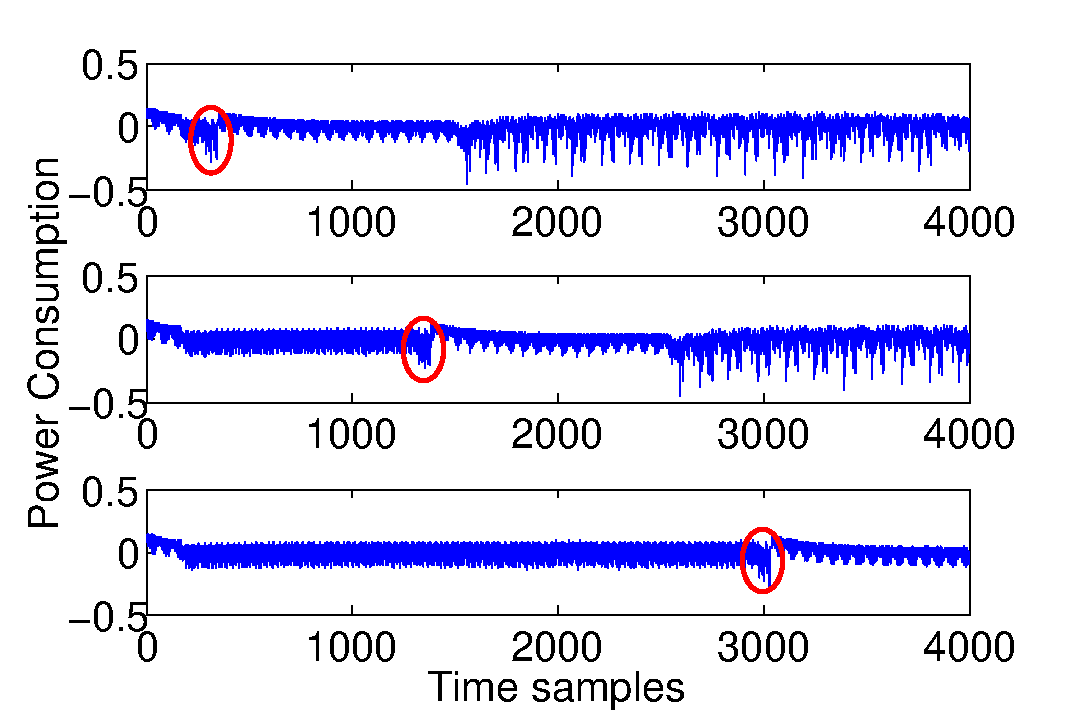
\includegraphics[width=0.5\textwidth]{CW-dataset/CW_shift_traces}
	\caption{An example of dummy operation (\textsf{nop}) randomly inserted before an informative leakage (in red). 
	Courtesy of Cagli \etal{}~\cite{cagli_convolutional_2017}.}
	\label{fig:dummy_op}
\end{figure}

\paragraph{Code Polymorphism.}
Due to the skyrocketing production of \gls{iot}, there is a need for the automated application of protections to improve products’ resistance against \gls{sca} while keeping the performance overhead sufficiently low. 
In this context, some recent works proposed compiler toolchains to automatically apply counter-measures such as bit-slice masking~\cite{belaid_tornado_2020} or a software hiding counter-measure called code polymorphism~\cite{belleville_automated_2019}. 
The working principle of the latter counter-measure relies on the execution of many variants of the machine code of the software device to protect, produced by a runtime code generator. 
The successive execution of many variants aims at producing variable side-channel traces in order to increase the difficulty to realize \gls{sca}. 
One must keep in mind that if code polymorphism is the only counter-measure applied to the target component, information leakage is still present in the side-channel traces. 
Yet, several works have shown the ability of code polymorphism and similar software
mechanisms to be effective in practice against \gls{vertical} \gls{sca}~\cite{agosta_code_2012,courousse_runtime_2016}, \ie{}, up to the point that the leakage characterization techniques presented in \autoref{sec:PoIs}, would not be able to detect information leakage in the traces, and that a \gls{cpa} would require several millions of queries whereas the same attack on the unprotected version of the targeted implementation succeeded within a few hundreds traces~\cite{agosta_meet_2015,belleville_automated_2019}.

We briefly describe the code polymorphism counter-measure applied by the toolchain used by Belleville \etal{}~\cite{belleville_automated_2019}. 
The compiler applies the counter-measure to selected critical parts of an unprotected source code: it inserts, in the target program, machine code generators, called \glspl{sgpc}, which can produce so-called polymorphic instances, \ie{}, many different but functionally-equivalent implementations of the protected components. 
At runtime, \glspl{sgpc} are regularly executed to produce new machine code instances of the polymorphic components. 
Thus, the device will behave differently after each code generation but the results of the computations are not altered. 
The toolchain supports several polymorphic code transformations, which can be selected separately in the toolchain, and most of them offer a set of configuration parameters. 
A developer can then set the level and the nature of polymorphic transformations, hence the amount of behavioral variability.

Hereafter, we detail some code transformations used in this thesis:
\begin{itemize}
	\item \textbf{Register shuffling}: the index of the general purpose callee saved registers are randomly permuted.
	\item \textbf{Instruction shuffling}: the independent instructions are randomly permuted.
	\item \textbf{Semantic variants}: some instructions are randomly replaced by another semantically equivalent (sequence of) instruction(s). 
	For example, variants of arithmetic instructions (e.g. \verb+eor+, \verb+sub+), remain arithmetically equivalent to the original instruction.
	\item \textbf{Noise instructions}: a random number of dummy instructions is added between the useful instructions in order to break the alignment of the leakage in the traces. 
	Noise instructions are interleaved with the useful ones by the instruction shuffling transformation.
\end{itemize}

We emphasize on the fact that the sensitive variables are only manipulated by the polymorphic instances (\ie{}, the generated machine code), and not by the \glspl{sgpc} themselves. 
\glspl{sgpc} are specialized code generators, and their only input is a source of random data (a \gls{prng} internal to the code generation runtime) driving the code generation. 
Hence, \glspl{sgpc} only manipulate instruction and register encodings, and never manipulate secret data. 
Thus, performing an \gls{sca} on side-channel traces of executions of \glspl{sgpc} cannot reveal a secret nor an information leakage. 
However, \glspl{sgpc} manipulate data that are related to the contents of the buffer instances, \ie{}, the structure of the generated code, the nature of the generated machine instructions (useful and noise instructions), \etc{} 
\gls{sca} performed on \gls{sgpc} traces could possibly be helpful to reveal sensitive information about the code used by the polymorphic instances, but to the best of our knowledge, there is no such work in the literature. 
As such, this research question is out of the scope of this thesis.

\section{Overview of the Used Datasets}
    \label{sec:datasets}
    %%%%%%%%%%%%%%%%%%%%%%%%%%%%%%%%%%%%%%%%%%%%%%%%%%%%%%%%%%%%%%%%%%%%%%%%%%%%%%%%
%                   DESCRIPTION OF THE DATASETS                                %
%%%%%%%%%%%%%%%%%%%%%%%%%%%%%%%%%%%%%%%%%%%%%%%%%%%%%%%%%%%%%%%%%%%%%%%%%%%%%%%%
We present in this section the different datasets of \gls{sca} traces which will be used for the experimental validation of our work in this thesis.
Those datasets cover a large spectrum of use cases.
Moreover, most of them are publicly available, which is of great interest for -- fair -- comparison with the state of the art.
Some of those datasets are used in several parts and contributions in this thesis.
That is why, for conciseness, we gather their description in a devoted section.

\subsection{Chip Whisperer Dataset (CW)}
\label{sec:dataset_cw}
This dataset has been used in the work we presented at \textsc{Ches} 2020~\cite{masure_comprehensive_2019}.
Although it does not depict the execution of a whole cryptographic primitive, it emulates the behavior of leakages of any secret-sharing scheme that may occur during the execution of assembly instructions in a software implementation.

\paragraph{The Target.}
The leakage traces represent the power consumption of a \textsf{XMEGA128D4} chip supported on a \textsf{Chip Whisperer Lite} board~\cite{oflynn_chip_2014}.
The firmware is directly written in assembly code.
A pseudo-code is provided in \autoref{alg:assembly}.
It consists in iteratively loading a byte of a \(16\)-byte plaintext array to a register of the \gls{mcu} in order to provoke a physical leakage, then setting the value of the byte to zero and then storing it back in \gls{ram}.
The operations are then repeated for each byte of the array.

\begin{algorithm}[ht]
    \caption{\textsf{loadData}}\label{alg:assembly}
    \begin{algorithmic}[1]
        \State LD   r0, X   \Comment{Loads the first byte in r0}
        \State CLR  r0      \Comment{Clears the register}
        \State ST   X, r0   \Comment{Stores 0 in the plaintext array}

        \State LD   r0, X   \Comment{Do it again to clear the bus}
        \State CLR  r0
        \State ST   X, r0

        \State LD   r0, X   \Comment{One more time to be sure}
        \State CLR  r0
        \State ST   X+, r0
    \end{algorithmic}
\end{algorithm}
\(500,000\) traces of \(2,500\) time samples each have been acquired, along with the corresponding bytes array denoted by \verb+plain[i]+, \(i \in \llbracket 0, 15 \rrbracket\). 
The complete acquisition has been done within \(15\) hours. 

\paragraph{Quick Analysis of the Traces.}
Since this dataset will mainly be used to investigate \gls{dl}-\gls{sca} in presence of secret-sharing, we would like to prevent any leakage jointly involving two bytes of the array.
\autoref{fig:cw_trace} shows an example of one trace acquired through the platform.
The 16 patterns denoting the execution of \autoref{alg:assembly} on each byte of the array are clearly distinguishable.
We provide the corresponding \gls{snr} in \autoref{fig:snr_cw} (top) in different colors for each byte.
In addition, we have also computed a \gls{snr} of order 2, that is, targeting the \verb+xor+ between two bytes, for any couple of bytes.
The absence of peaks tends to confirm that there is no undesirable leakage, at least involving such a \verb+xor+.
However, a leakage between two bytes involving another relationship than a \verb+xor+ might still be informative, this does not allow to draw a sharp conclusion.
Emphasizing such a leakage would require many more traces to reach a significant conclusion.
That is why we let open this eventuality, although we remain confident that it is not likely to happen.
\begin{figure}[ht]
    \centering
    \begin{subfigure}{\textwidth}
        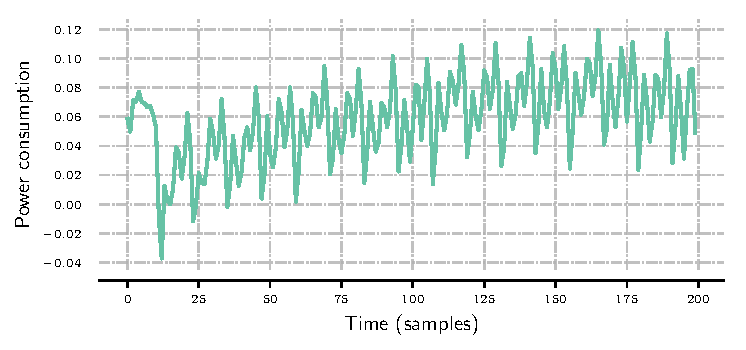
\includegraphics[width=\textwidth]{CW-dataset/exp_trace}
        \caption{Illustration of one trace}
        \label{fig:cw_trace}
    \end{subfigure}
    \begin{subfigure}{\textwidth}
        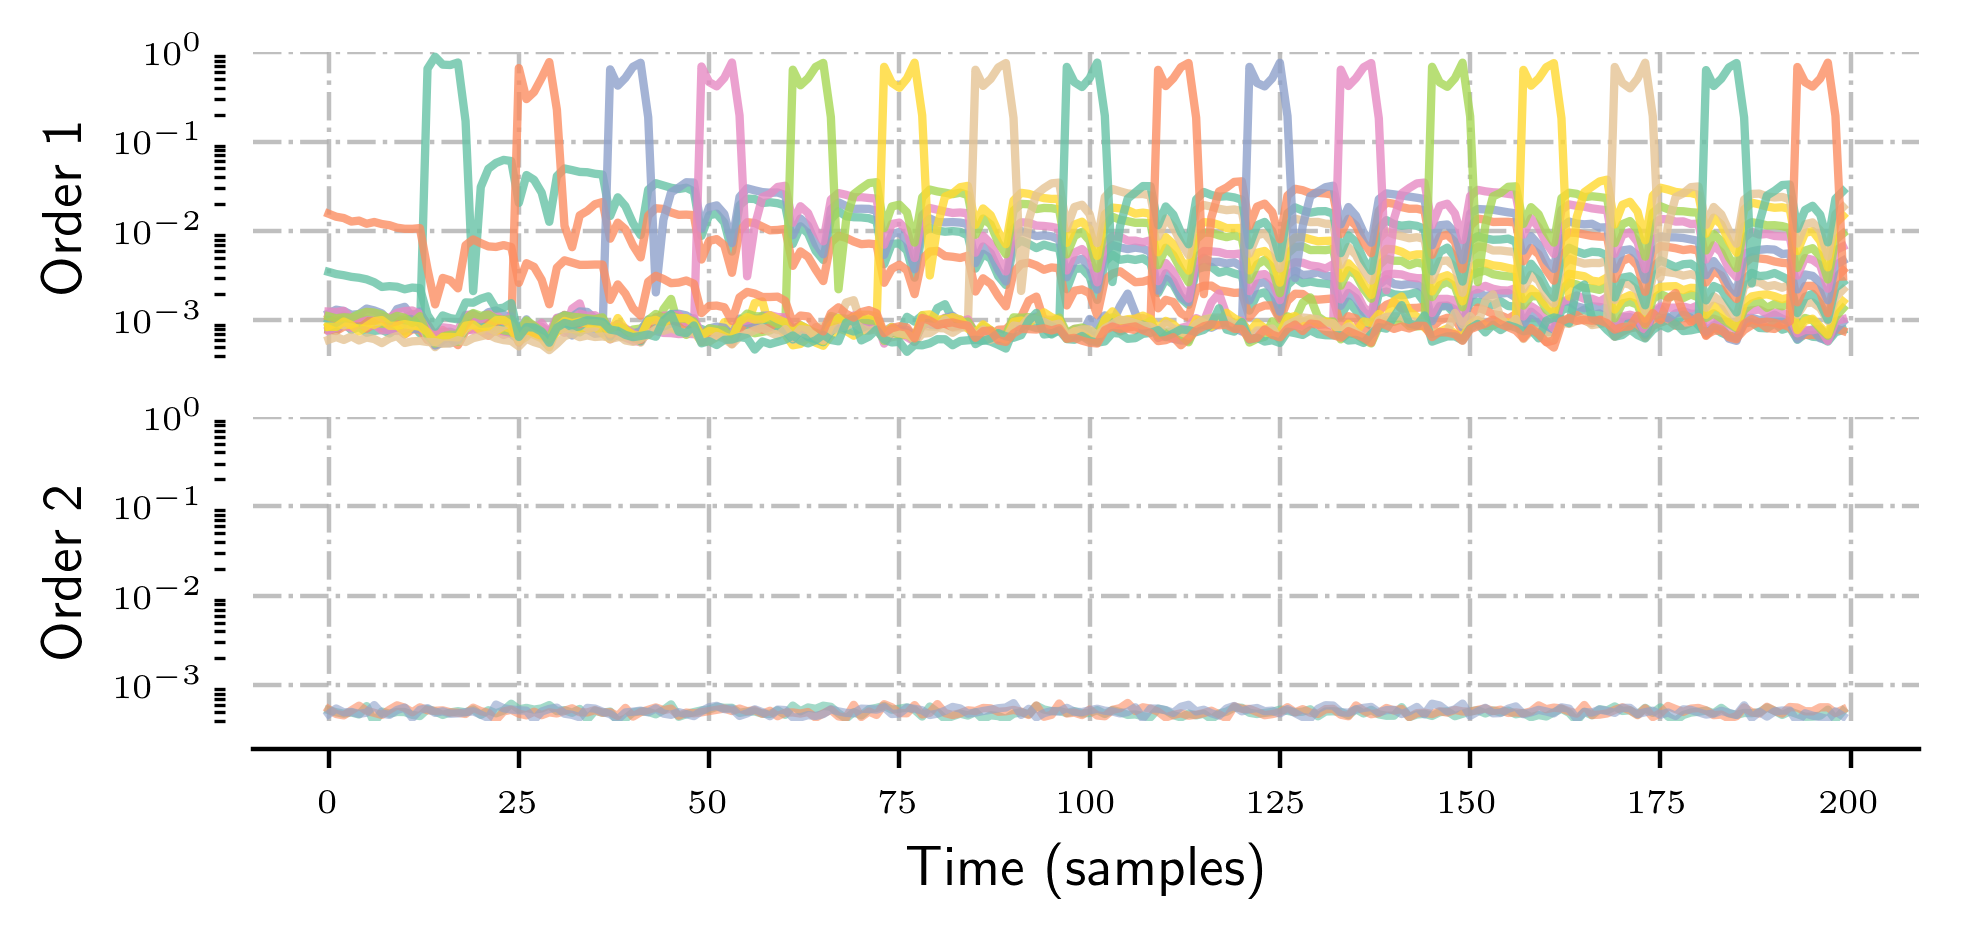
\includegraphics[width=\textwidth]{CW-dataset/snr_reduce.png}
        \caption{The \glspl{snr} of order 1 and 2 (in log scale).}
    \end{subfigure}
    \caption{The CW dataset.}
    \label{fig:snr_cw}
\end{figure}

\subsection{The ASCAD Dataset}
\label{sec:ascad}
The \gls{ascad} dataset has been introduced in 2018 by Benadjila \etal{}~\cite{prouff_study_2018} to provide the \gls{sca} community a benchmark to investigate and compare \gls{dl}-based attacks.
In particular, the aim is to assess to what extent deep learning is relevant to mount attacks against protected implementations.

\paragraph{The Target.}
The target is a protected software \gls{aes}-128 implementation running over an \textsf{ATMEGA-8515}, which has an 8-bit \textsf{AVR} architecture.
The software aims at protecting against first-order \gls{sca}, by using a Boolean secret-sharing scheme based on the table re-computation method (\cf{} \autoref{algo:table_recomputation}), although the first two bytes of the \gls{aes} state are not protected, for the sake of comparison.
Typically, the targeted variable on this dataset is the third byte of the state, at the output of the \(\Sbox\) in the first round, \ie{}, \(\Z = \fonction{\Sbox}{\p[3] \oplus \key[3]}\).
The dataset provides \(60, 000\) traces, where \(\numTracesProf = 50, 000\) traces are used for profiling and \(\numTracesVal = 10, 000\) for validation, \ie{}, for emulating attacks phases -- see \autoref{sec:estimate_practice}.
For both datasets, the same fixed key has been used, while the plaintexts and the shares have been randomly drawn.%
\footnote{
    Since the first release, a new version of the traces has been published, using a random key in the profiling traces, which are besides twice larger.
    This version is not investigated in this thesis.
}
Whereas the whole traces, focused on the first \gls{aes} round are made of \(100,000\) time samples, this thesis will focus on the chunk corresponding to the interval \(\llbracket 45,400; 46,100\rrbracket\), \ie{}, \(\traceLength = 700\).
This window corresponds to the joint leakage of \(\Z \oplus \rout\) and \(\rout\).
Three versions of this dataset are available: the first one provides the traces as is, whereas the second and third ones provide the same traces on which an artificial shift of maximum amplitude of respectively 50 and 100 points has been applied.
The traces are publicly available at \url{https://github.com/ANSSI-FR/ASCAD}.

\paragraph{Quick Analysis of the Traces.}
A characterization with the statistical methods presented in \autoref{sec:PoIs} is provided in \autoref{fig:charac_ascad}.
\autoref{fig:charac_ascad_t_test} depicts the characterization thanks to a T-test, while \autoref{fig:charac_ascad_snr} depicts the characterization done with a \gls{snr}.
\begin{figure}
    \centering
    \begin{subfigure}{0.49 \textwidth}
        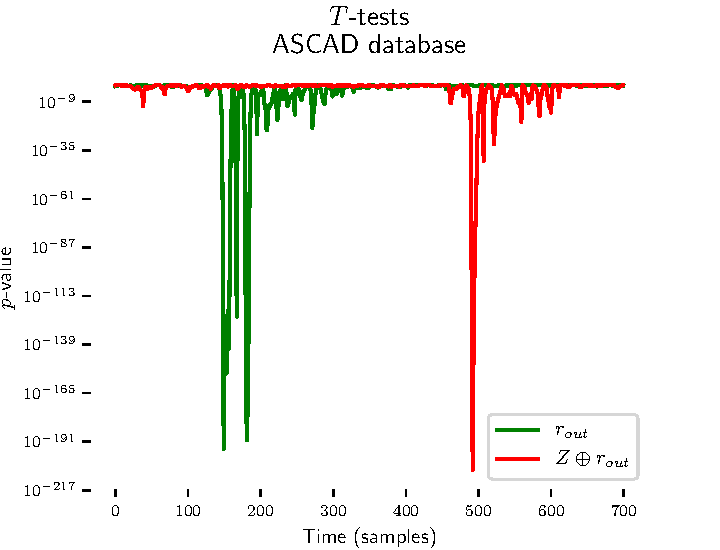
\includegraphics[width=\textwidth]{ASCAD/ttest_m_and_zxm}
        \caption{T-test}
        \label{fig:charac_ascad_t_test}
    \end{subfigure}
    \begin{subfigure}{0.49 \textwidth}
        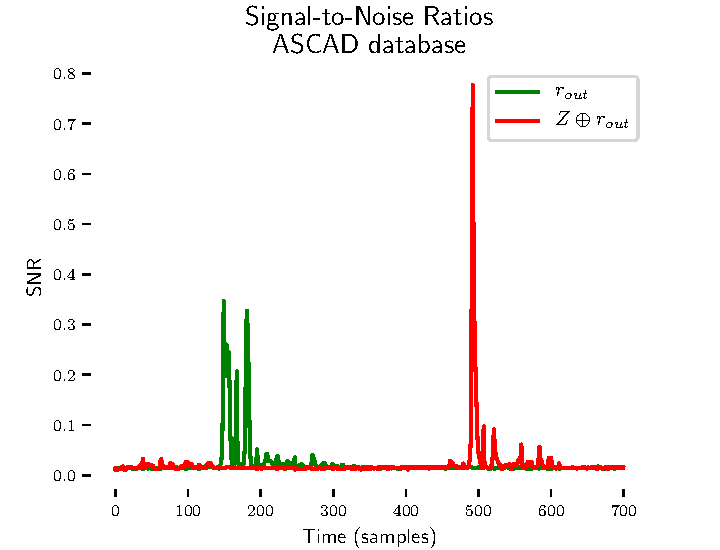
\includegraphics[width=\textwidth]{ASCAD/snr_m_and_zxm}
        \caption{\gls{snr}}
        \label{fig:charac_ascad_snr}
    \end{subfigure}
    \caption{Leakage characterization with statistical tools over the \gls{ascad} dataset, without artificial shift.}
    \label{fig:charac_ascad}
\end{figure}
On those two plots, the green peaks emphasize the leakage of the random share \(\rout\), while the red peaks denote the leakage of the output of the re-computed \(\Sbox\), namely \(\Z \oplus \rout\).
The recombination of the two leakages would give access to information about the sensitive variable \(\Z\), which might be a privileged target for an attacker.

Nevertheless the latter characterization is successful because we have assumed the attacker (or the evaluator) to have access to the values of the random share \(\rout\).
This assumption turns out to be critical, as pointed in \autoref{fig:charac_ascad_mask}.
This figure denotes the \gls{snr} directly computed over the sensitive variable \(\Z\), \ie{}, without knowledge of the random share \(\rout\).
One can see on the plot that no clear peak appears, and that the level of \gls{snr} is much lower than in \autoref{fig:charac_ascad_snr}.
This shows that without knowledge of the random share \(\rout\), the \gls{snr} becomes unable to localize any \gls{poi}.

Likewise, the random shift artificially applied to the traces occurs a similar effect on the \gls{snr} computation, as shown in \autoref{fig:charac_ascad_shift}.
Here again, no clear peak is emphasized on the plot.
Hence, no \gls{poi} selection can be done on the traces thanks to statistical tools usually used for characterization.
A way to circumvent this difficulty will be presented in \autoref{chap:gradient_viz}.

\begin{figure}
    \centering
    \begin{subfigure}{0.49 \textwidth}
        \includegraphics[width=\textwidth]{ASCAD/snr_raw}
        \caption{Characterization without knowledge of the secret shares.}
        \label{fig:charac_ascad_mask}
    \end{subfigure}
    \begin{subfigure}{0.49 \textwidth}
        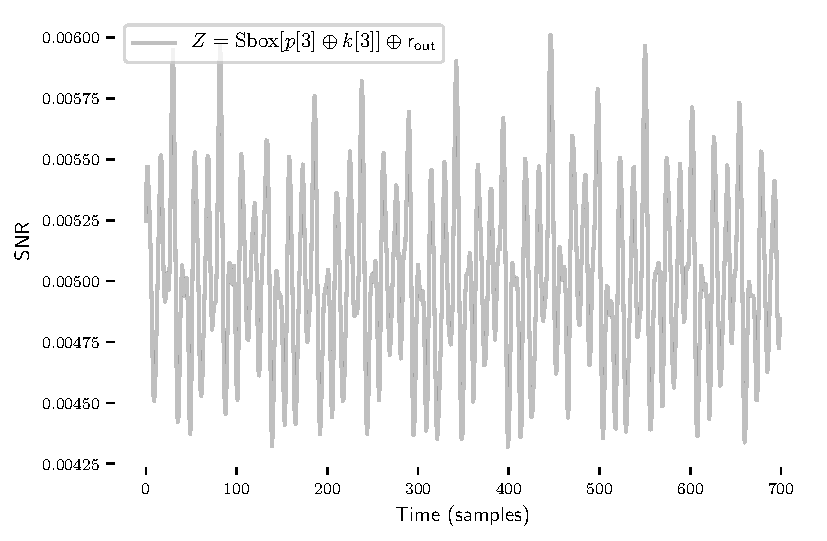
\includegraphics[width=\textwidth]{ASCAD/snr_desync50}
        \caption{Characterization on randomly shifted traces (\(T=50\)).}
        \label{fig:charac_ascad_shift}
    \end{subfigure}
    \caption{Effect of the counter-measures to the characterization on the \gls{ascad} dataset.}
    \label{fig:charac_ascad_cm}
\end{figure}

\subsection{Random Delay Dataset (AES-RD)}
\label{sec:aesrd}
The \gls{aesrd} dataset has been released, following the works of Coron \etal{} on the insertion of random delays in the implementation of a software AES, as a way to implement the dummy operation insertion~\cite{coron_random_2009,coron_random_2010}.
In a nutshell, it consists in drawing -- thanks to the \gls{prng} -- a random number of cycles during which a loop will iterate.

\paragraph{The Target.}
The target smart-card is an 8-bit \textsf{Atmel AVR} micro-controller, protected by a random delay counter-measure, which has an effect on the misalignment of the traces, making some attacks such as with \glspl{gta} much harder.
The targeted variable is the output of the first \(\Sbox\).
The dataset is publicly available at \url{https://github.com/ikizhvatov/randomdelays-traces}.
\(50,000\) traces of \(\traceLength = 3,500\) time samples each are provided, denoting the power consumption of the target.
These power traces have been previously compressed by selecting 1 sample (peak) from each \gls{cpu} clock cycle.
At least the first (non-dummy) \gls{aes} round is covered.
In this thesis, we split the dataset into \(\numTracesProf = 40,000\) profiling traces and \(\numTracesVal = 10,000\) validation traces.

\paragraph{Quick Analysis of the Traces.}
We provide in \autoref{fig:snr_aes_rd} an example of trace from the dataset (top), along with a characterization with \gls{snr} over the whole dataset (bottom).
\begin{figure}
    \centering
    \includegraphics[width=\textwidth]{AES-RD/snr}
    \caption{Top: An example of a trace from the \gls{aesrd} dataset.
    Bottom: the \gls{snr} computed over the whole dataset.}
    \label{fig:snr_aes_rd}
\end{figure}
As expected, due to the misalignment effect of the random delay counter-measure, no peak denoting a leakage is emphasized.
This confirms that either a pre-processing phase including re-alignment or the use of a misalignment-resilient methods is necessary to deal with those traces.

\subsection{AES on FPGA (AES-HD)}
\label{sec:aeshd}
The \gls{aeshd} dataset has been released by Picek \etal{} at \textsc{Ches} 2019~\cite{picek_curse_2019}, in order to introduce a dataset of \gls{sca} traces targeting a hardware implementation whereas the majority of the public datasets are focused on software implementations.
Moreover, this dataset is an example of use-case where the targeted sensitive variable comes from the last round of the \gls{aes} encryption.

\paragraph{The Target.}
We recall hereafter the description provided by Picek \etal{} in their paper.
This is an ``unprotected implementation of \gls{aes}, written in \gls{vhdl} in a round based architecture taking 11 clock cycles for each encryption.
The design was implemented on a \textsf{Xilinx Virtex-5} \gls{fpga} of a \textsf{SASEBO GII} evaluation board. 
Side-channel traces were measured using a high sensitivity near-field \gls{em} probe,
placed over a decoupling capacitor on the power line.''
The dataset is publicly available at \url{https://github.com/AESHD/AES_HD_Dataset}.

The authors recommend to use an intermediate leakage model \(\varphi\) corresponding to the Hamming distance between the targeted byte of the state before applying the \(\Sbox\) of the last round, and the final ciphertext byte.
In the following of this thesis, we will rather target the input of the last \(\ark\), without considering any prior leakage model.

\paragraph{Quick Analysis of the Traces.}
\autoref{fig:snr_aes_hd} provides a brief insight of the traces.
\begin{figure}
    \centering
    \includegraphics[width=\textwidth]{AES-HD/snr}
    \caption{Top: one trace of the \gls{aeshd} dataset.
    Bottom: The SNR computed over the whole dataset.}
    \label{fig:snr_aes_hd}
\end{figure}
One can guess 10 similar patterns corresponding to the 10 rounds of \gls{aes}.
The peak of \gls{snr} appears on the last pattern, confirming that the targeted sensitive variable is an intermediate computation of the last round.
Although the peak is clearly distinguishable, one may remark that the peak is at approximately \(0.15\), which is lower than the preceding \glspl{snr} observed in \autoref{fig:snr_cw} and \autoref{fig:charac_ascad_snr}.
This is expected since hardware implementations are known to usually leak less information.


\subsection{Polymorphism Dataset}
\label{sec:claps_ds}
In \autoref{chap:dl_sca_practice}, we will present the investigations conducted on the security of the code polymorphism counter-measure proposed by Belleville \etal{}~\cite{belleville_automated_2019}.
To this end, we conducted an acquisition campaign of \gls{sca} traces over two out of the 15 implementations used in their benchmarks, namely the \aeshuitbit{} and the \mbedTLS{} that we briefly describe hereafter, along with the details of the experimental setup and a preliminary analysis.

\paragraph{The \mbedTLS{} Implementation.}
This \(32\)-bit implementation of \gls{aes} from the \textsf{ARM} library~\cite{mbed_tls_code} follows the so-called \emph{T-table} technique~\cite{AES_rijndael_2002}: the \(16\)-byte state of \gls{aes} is encoded into four \verb+uint32_t+ variables, each representing a column of the state.
Each round of the \gls{aes} is done by applying four different constant \glspl{lut} stored in flash memory.

\paragraph{The \aeshuitbit{} Implementation.}
This is a simple software unprotected implementation of \gls{aes} written in \textsf{C}, and manipulating only variables of type \verb+uint8_t+, similar to \cite{SmallportableAES1282020}.
The \(\sub\) operation is computed byte-wise thanks to a \gls{lut}, stored in \gls{ram}.
This reduces information leakage on memory accesses, compared to the use of the same \gls{lut} stored in flash memory.

\paragraph{Target Device.}
We ran the different AES implementations on an \textsf{STM32 NUCLEO F303} board, embedding an \textsf{ARM Cortex-M4} \(32\)-bit core~\cite{STMicroelectronicsNUCLEOF303RE}.
This device does not provide any hardware security mechanisms against side-channel attacks.
This core originally operates at \(72\)~MHz, but the core frequency was reduced to \(8\)~MHz for the purpose of side-channel measurements.
The target is similar to the one used by Belleville \etal{}~\cite{belleville_automated_2019}, who considered a \textsf{Cortex-M3} core running at \(24\)~MHz.
These two micro-controllers have an in-order pipeline architecture, but with a different pipeline organization.
Thus, we cannot expect those two platforms to exhibit the same side-channel characteristics.
However, our experience indicates that these two experimental setups would lead to similar conclusions regarding the attacker models considered in our study.
Similar findings on similar targets have also been reported by Heuser \etal{}~\cite{heuser_physical_2020}.
Therefore, we assume that the differences of side-channel characteristics between our targets and the Belleville \etal{}'s ones should not induce major differences in the results of such side-channel analysis.

\paragraph{Configuration of the Code Polymorphism Counter-Measure.}
For each evaluated implementation, the code polymorphism counter-measure is applied with a level corresponding to the configuration ``\textsf{high}'' described by Belleville \etal{}~\cite{belleville_automated_2019}: all the polymorphic code transformations  are activated, the number of inserted noise instructions follows a probability distribution based on a truncated geometric law.
The dynamic noise is activated and \glspl{sgpc} produce a new polymorphic instance of the protected code for \emph{each} execution (\ie{}, the regeneration period is set to 1).

\paragraph{Acquisition Setup.}
\label{sec:setup}
We measured \gls{sca} traces corresponding to \gls{em} emanations with an \gls{em} probe \textsf{RF-B 0.3-3} from Langer, equipped with a pre-amplifier, and a \textsf{Rohde \& Schwarz RTO} \(2044\) oscilloscope with a \(4\) GHz bandwidth and a vertical resolution of \(8\)~bits.
We set the sampling rate to \(200\)~MS/sec., with the acquisition mode ``\emph{peak-detect}' which collects the minimum and the maximum voltage values over each sampling period.
We first verify that our acquisition setup is properly set.
This is done by acquiring several traces where the code polymorphism is de-activated.
Thus, we can verify that those traces are synchronized.
Then, computing the T-test (\cf{} \autoref{sec:PoIs}) enables to quickly\footnote{\ie{}, faster than with a \gls{snr} computation.} assess whether the probe is correctly positioned and the sampling rate is high enough.
Then, after re-activating the code polymorphism, \(100,000\) profiling traces are acquired for each target implementation.
Each acquisition campaign lasts about \(12\) hours.

\paragraph{Preliminary Analysis of the Traces.}
\label{sec:visual_inspect}
We detail hereafter a preliminary analysis of the acquired traces.
The aim is to restrict as much as possible the target region acquired to a window covering the entire first \gls{aes} round.
Therefore there would not be any loss of informative leakage about the sensitive intermediate variable targeted in those experiments.
In addition to that, a uni-variate leakage assessment, by computing the \gls{snr}, is provided hereafter in order to verify that there is no trivial leakage.

\subparagraph{\mbedTLS{}.}
We ran some preliminary acquisitions on \(10^7\) samples, in order to visualize all the execution.
We could clearly distinguish the \gls{aes} execution with sparse \gls{em} peaks, from the call to the \gls{sgpc} with more frequent \gls{em} peaks.
This enabled to focus on the first \(10^6\) samples of the traces corresponding to the \gls{aes} execution.

Actually, the traces restricted to the \gls{aes} execution seem to remain globally the same between each other, up to local elastic deformations along the time axis.
This is in line with the expected effect of code polymorphism, since it involves transformations at the machine code level.
Likewise, \(10\) patterns could be distinguished on each trace, which were clues to expect that it would correspond to the \(10\) rounds of \gls{aes}. 
That is how we could restrict again our target window to the first round, up to comfortable margins because of the misalignment effect of code polymorphism.
This represents \(80,000\) samples.
An illustration of two traces restricted to the first round is given by \autoref{fig:observations_v1} (top).%
\footnote{Here the first \(20\ \mu\)s of both traces correspond to a non-critical part of the implementation, probably due to the \gls{os} of the chip.
Hence the apparent synchronization here.}

\begin{figure}[t]
	\centering
	\includegraphics[width=\textwidth]{CLAPS/v1/snr_raw}
	\caption{Acquisitions on the \mbedTLS{} implementation.
	Top: two traces containing the first AES round.
	Bottom: SNR computed on the \(100,000\) profiling traces.}
	\label{fig:observations_v1}
\end{figure}

% SNR computation
The \gls{snr} denoting here the potential uni-variate leakage of the first output byte of the \sub{} operation is computed based on the \(100,000\) acquired profiling traces, and is plotted in \autoref{fig:observations_v1} (bottom).
No distinguishing peak can be observed, which confirms the soundness of code polymorphism against attacks requiring the \glspl{poi} of the raw traces to be aligned with each other, \eg{}, the \gls{cpa} or the \gls{gta}.

% Realignment
However, we observe in each trace approximately 16 \gls{em} peaks corresponding to the number of memory accesses to the \glspl{lut} per encryption round.
These memory accesses are known to carry sensitive information.
This suggests that a trace re-alignment on \gls{em} peaks might be relevant to successfully achieve such attacks.%
\footnote{
    A re-alignment process is proposed in \autoref{sec:method}.
}

\subparagraph{\aeshuitbit{}.}
We proceed in the same way for the evaluation of \aeshuitbit{} implementation.
As with the \mbedTLS{} traces, we could identify \(10\) successive patterns likely to correspond to the \(10\) \gls{aes} rounds.
Therefore we reduce the target window at the oscilloscope to the first \gls{aes} round, which represents \(160,000\)-dimensional traces plotted in \autoref{fig:observations_v2} (top).
\begin{figure}[t]
	\centering
	\includegraphics[width=\textwidth]{CLAPS/v2/snr_raw}
	\caption{Acquisitions on the \aeshuitbit{} implementation.
	Top: two traces containing the first \gls{aes} round.
	Bottom: \gls{snr} computed on the \(100,000\) profiling traces.}
	\label{fig:observations_v2}
\end{figure}
This growth in the size of the traces is expected, since the naive \aeshuitbit{} implementation is not optimized to be fast, contrary to the \mbedTLS{} one.

Yet, here the peaks are hardly distinguishable from the level of noise.
This is expected, due to the \glspl{lut} being moved from the flash memory to the \gls{ram}.
As a consequence, the memory accesses are less remarkable.
That is why a trace re-alignment does not seem relevant here.

Finally, \autoref{fig:observations_v2} (bottom) shows the SNR on the raw traces, ensuring once again that no trivial leakage can be exploited to recover the secret key.

\section{Conclusion}
    In this chapter, we have presented the attack scenario considered in this thesis.
    Starting from the so-called ``gray-box'' scenario (\autoref{sec:attack_scenario}), the latter one may be augmented with a preliminary profiling phase with the help of an open-sample clone device of the target.
    This leads to the profiling attack scenario presented here (\autoref{fig:prof_scenario}).
    We have stated that in this scenario, the attack is jointly defined by two elements: the choice of the distinguisher (\autoref{def:distinguisher}), and the design of the leakage model.
    In particular, the profiling phase aims at estimating the true leakage model as precisely as possible, in order to reach a satisfying solution of the fundamental goal of the \gls{sca} evaluator, as stated by \autoref{final_task} and \autoref{thm:opt_sol_prob1}.

    From a practical perspective, the design of the leakage model often requires a preliminary dimensionality reduction, \eg{}, with the help of a \glspl{poi} selection method.
    We have briefly presented two statistical tools in \autoref{sec:PoIs} enabling such a selection, illustrated in the presentation of the datasets investigated through the experiments of this thesis (\autoref{sec:datasets}).

    Regarding the way that the vulnerabilities of a leaky device could be exploited by potential attackers, a developer is not unarmed.
    Hopefully, he can indeed control the quantity of informative leakage resulting from the execution of the targeted implementation through several means, namely the randomization of the sensitive data encoding (\aka{} secret-sharing, \autoref{sec:masking}) or the randomization of the operations (\aka{} hiding, \autoref{sec:hiding}).
    Provided with those counter-measures, the developer has the power to trade off runtime and memory performance against security.

    Yet, several questions remain unanswered at the end of this chapter.
    Indeed, although we have presented the attack techniques against unprotected implementations, we did not thoroughly discussed how the attacker can adapt its techniques -- or even adopt new ones -- to the counter-measures presented so far.
    This issue will be investigated in \autoref{chap:ches_20}, when we will address the efficiency of neural networks as a way to modelize the posterior conditional \gls{pmf} of the leakage, for a protected implementation.

    Besides, we have quickly mentioned to what extent the machine learning techniques can be integrated to the profiling attack framework presented in this chapter.
    In \autoref{chap:machine_learning}, we will dive in more details about this fact, and we will see that the profiling attack framework and the machine learning framework are somehow intertwined.